
\section{$\widehat{\psi}$ 的性质：\trGluing{}的唯一性}
\label{sec:uniqueness-gluing}

我们刚刚证明了：破碎\trTrajectory{} $(\widehat{u},\widehat{v})\in\scr{L}(x,y)\times\scr{L}(y,z)$
是\trEmbedding{}在 $\overline{\scr{L}}(x,z)$ 中的一个区间的端点，此区间的内部是 $\scr{L}(x,z)$ 的一个\trConnectedComponent{}。这还不足以断定 $\overline{\scr{L}}(x,z)$ 是一个维数为 $1$ 的\trManifoldWithBoundary，正如\cref{fig:two-arcs-same-endpoint}所显示的那样。

\begin{figure}[htbp]
\centering
\begin{tikzpicture}[line cap=round,line join=round]
\draw[dashed,thick] (-2.6,1.05) .. controls (-1.7,0.62) and (-0.9,0.32) .. (0.15,0.12);
\draw[thick] (-1.7,-1.6) .. controls (-1.15,-0.6) and (-0.6,0.1) .. (0.15,0.12);
\draw[fill] (0.15,0.12) circle (0.02);
\node at (0.95,0.12) {$(\widehat{u},\widehat{v})$};
\end{tikzpicture}
\caption{}
\label{fig:two-arcs-same-endpoint}
\end{figure}

我们还必须证明：在 $\overline{\scr{L}}(x,z)$ 中逼近 $(\widehat{u},\widehat{v})$ 的唯一途径（除了常值序列之外）就是经由我们刚才构造的那个区间。这正是\cref{thm:gluing-psi}的最后一条断言（它换了一种说法表达了\trMorseComplex{}中的相应陈述，即\cref{thm:gluing-embedding}）：如果 $\scr{L}(x,z)$ 中的一个序列\trConvergence{}到 $(\widehat{u},\widehat{v})$，那么它就在 $\widehat{\psi}$ 的像之中。

困难来自下面这一点：\trGluing{}的构造与映射 $\widehat{\psi}$ 的构造都依赖于若干任意的选取。例如，考虑一个 $\cC^{\infty}$ 类的函数 $\nu\colon\RR_{+}\to\RR_{+}$，满足 $\lim_{\rho\to+\infty}\nu(\rho)=+\infty$。在我们所用过的那些公式里，把 $v(s-\rho)$ 换成 $v(s-\nu(\rho))$，就可以定义一个\trPregluing{} $w_{\nu,\rho}$：\footnote{译注：原书下式末行印作 $v(s-\nu(\rho))$，未带自变元 $t$；按第一行 $u(s+\rho,t)$ 以及 §9.3 中 $w_{\rho}$ 原式末行 $v(s-\rho,t)$ 的口径，疑应为 $v(s-\nu(\rho),t)$，此处径改。——译者注}
\[
w_{\nu,\rho}(s,t)=
\left\{
\begin{array}{ll}
u(s+\rho,t) & \text{若 } s\le -1\\[10pt]
\begin{aligned}
\exp_{y(t)}\Bigl(\beta^{-}(s)\exp_{y(t)}^{-1}u(s+\rho,t)\\
+\ \beta^{+}(s)\exp_{y(t)}^{-1}v(s-\nu(\rho),t)\Bigr)
\end{aligned}
& \text{若 } s\in[-1,1]\\[10pt]
v(s-\nu(\rho),t) & \text{若 } s\ge 1\text{。}
\end{array}
\right.
\]
我们请读者验证：从 $w_{\nu,\rho}$ 出发重做\trGluing{}的构造，就会得到一个连续映射
\[
\psi_{\nu}\colon[\rho_{\nu},+\infty[\ \longrightarrow\scr{M}(x,z)
\]
使得
\[
\lim_{\rho\to+\infty}\pi\circ\psi_{\nu}(\rho)=(\widehat{u},\widehat{v})\text{。}
\]
他们随后还将验证：若 $\nu$ 是递增的，那么映射 $\widehat{\psi}_{\nu}=\pi\circ\psi_{\nu}$ 就是一个\trInjective{}\trImmersion。$\widehat{\psi}$ 的情形正是 $\nu=\mathrm{Id}$ 的情形。

为了避免\cref{fig:two-arcs-same-endpoint}中所勾画的那个局面，我们需要保证：新映射 $\widehat{\psi}_{\nu}$ 的像（对充分大的 $\rho$）含于先前构造的\trGluing{} $\widehat{\psi}=\widehat{\psi}_{\mathrm{Id}}$ 的像之中。这将是我们的证明的第一步，整个证明将由四个步骤组成：

（1）第一步就是我们刚才所描述的那一步，它在于证明下面这个结果。

\begin{proposition}\label{thm:psinu-image-contained}
设 $\nu\colon\RR_{+}\to\RR_{+}$ 是一个 $\cC^{\infty}$ 类的递增函数，满足 $\lim_{\rho\to+\infty}\nu(\rho)=+\infty$。那么存在一个 $\rho_{\nu}>0$，使得对 $\rho\ge\rho_{\nu}$，我们有 $\widehat{\psi}_{\nu}(\rho)\in\mathrm{Im}(\widehat{\psi})$。
\end{proposition}

（2）第二步：考虑一个在 $\overline{\scr{L}}(x,z)$ 中趋于 $(\widehat{u},\widehat{v})$ 的序列 $(\ell_{n})_{n\in\NN}$。与\cref{thm:gluing-psi}中一样，我们想证明：对充分大的 $n$，$\ell_{n}\in\mathrm{Im}(\widehat{\psi})$。

\begin{remark}\label{thm:subsequence-suffices}
只需证明：存在一个子序列 $(\ell_{n_{k}})_{k\in\NN}$，使得对充分大的 $k$，$\ell_{n_{k}}\in\mathrm{Im}(\widehat{\psi})$。
\end{remark}

事实上，假定\cref{thm:gluing-psi}的结论不成立。那么我们就有一条子序列 $\ell_{n_{k}}$，它不在 $\widehat{\psi}$ 的像之中，却在 $\overline{\scr{L}}(x,z)$ 中趋于 $(\widehat{u},\widehat{v})$。在这种情形下，从某一项起，我们可以抽取一个含于 $\mathrm{Im}(\widehat{\psi})$ 之中的子序列，这就给出一个矛盾。

在下面的诸陈述中，凡是涉及序列 $(\ell_{n})_{n\in\NN}$ 的结论，都是在必要时抽取一个子序列之后成立的。在这第二步中，我们证明下面这个结果。

\begin{proposition}\label{thm:lift-exp-decay}
存在 $\ell_{n}$ 的一个\trLift{} $\widetilde{\ell}_{n}\in\scr{M}(x,z)$ 与一个 $\cC^{\infty}$ 类的递增函数 $\nu\colon\RR_{+}\to\RR_{+}$，$\lim_{\rho\to+\infty}\nu(\rho)=+\infty$，使得对每个 $(s,t)\in\RR\times S^{1}$，
\[
\widetilde{\ell}_{n}(s,t)=\exp_{w_{\nu,\rho_{n}}(s,t)}Y_{n}(s,t)\text{，}
\]
其中序列 $(\rho_{n})$ 趋于 $+\infty$，而 $Y_{n}\in w_{\nu,\rho_{n}}^{\star}TW$ 满足
\[
\lim_{n\to+\infty}\|Y_{n}\|_{\infty}=0\text{。}
\]
\end{proposition}

范数 $\|Y_{n}\|_{\infty}$ 是这样计算的：借助我们所固定的 $W$ 在 $\RR^{m}$ 中的\trEmbedding{}以及 $\RR^{m}$ 上的\trEuclidean{}范数，把 $Y_{n}$ 视为映射
\[
Y_{n}\colon\RR\times S^{1}\longrightarrow\RR^{m}
\]
来计算。

（3）第三步是技术上最棘手的一步。沿用前面的记号，我们证明下面这个结果。

\begin{proposition}\label{thm:yn-w1p}
\trVectorField{} $Y_{n}$ 满足：$Y_{n}\in W^{1,p}(w_{\nu,\rho_{n}}^{\star}TW)$ 对每个 $p>2$ 成立。此外，$\lim_{n\to+\infty}\|Y_{n}\|_{W^{1,p}}=0$。
\end{proposition}

我们回顾一下，第一条断言不过是说
\[
Y_{n}\in W^{1,p}(\RR\times S^{1};\RR^{m})
\]
（解释见\cref{sec:banach-manifold-p1p}）。

（4）在第二步与第三步之后，我们手中便有一个序列 $\widetilde{\ell}_{n}$，它与借助\trPregluing{} $w_{\nu,\rho_{n}}$ 由\trNewton--\trPicard{}方法产出的一个解具有相同的形状。我们回顾一下：为了从 $w_{\nu,\rho_{n}}$ 出发应用\trNewton--\trPicard{}方法（\cref{thm:abstract-newton-picard}），我们必须先把 $W^{1,p}(\RR\times S^{1};\RR^{2n})$ 分解成一个\trDirectSum{} $\operatorname{Ker}(L_{\rho_{n}})\oplus W_{\rho_{n}}^{\perp}$，这个\trDirectSum{}现在依赖于 $n$（即所论的 $\rho_{n}$ 的下标），并且在这个\trDirectSum{}中，$\operatorname{Ker}(L_{\rho_{n}})$ 的维数为 $2$（参见\cref{thm:lrho-lower-bound}的诸推论）。利用一个\textbf{\trContractingMap}（contracting map）
\[
\varphi\colon W_{\rho_{n}}^{\perp}\cap B(0,\varepsilon_{0})\longrightarrow W_{\rho_{n}}^{\perp}\cap B(0,\varepsilon_{0})
\]
（其中 $\varepsilon_{0}>0$ 不依赖于 $n$），我们找到一个唯一的 $\gamma_{n}\in W_{\rho_{n}}^{\perp}\cap B(0,\varepsilon_{0})$，使得 $\exp_{w_{\nu,\rho_{n}}}\gamma_{n}\in\scr{M}(x,z)$：这个 $\gamma_{n}$ 就是映射 $\varphi$ 的唯一\trFixedPoint。细心的读者想必已经注意到：我们借助映射
\[
i\colon W^{1,p}(\RR\times S^{1};\RR^{2n})\longrightarrow w_{\nu,\rho_{n}}^{\star}TW
\]
（它由沿 $w_{\nu,\rho_{n}}$ 的一个固定的酉\trTrivialization{}所定义），把 $W^{1,p}(\RR\times S^{1};\RR^{2n})$ 与 $w_{\nu,\rho_{n}}^{\star}TW=T_{w_{\nu,\rho_{n}}}\scr{P}(x,z)$ 等同了起来。

由于 $\|Y_{n}\|_{W^{1,p}}$ 趋于 $0$，故对充分大的 $n$，$Y_{n}$ 落在球 $B(0,\varepsilon_{0})$ 之中。特别地，$Y_{n}\in h_{n}+W^{\perp}$，其中 $h_{n}\in B(0,\varepsilon_{0})\cap\operatorname{Ker}L$ 满足 $\lim_{n\to+\infty}\|h_{n}\|_{W^{1,p}}=0$。

\begin{figure}[htbp]
\centering
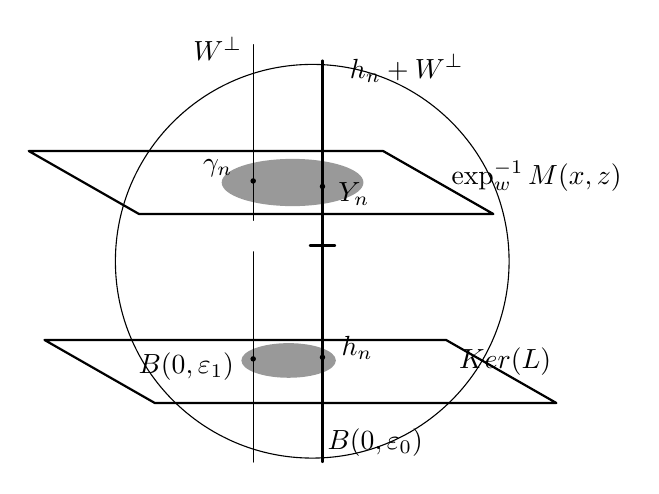
\begin{tikzpicture}[line cap=round,line join=round]
\draw (0.25,0.6) circle (2.5);
\draw[thick] (-3.15,-0.4) -- (1.95,-0.4) -- (3.35,-1.2) -- (-1.75,-1.2) -- cycle;
\node at (2.7,-0.68) {$\operatorname{Ker}(L)$};
\draw[thick] (-3.35,2.0) -- (1.15,2.0) -- (2.55,1.2) -- (-1.95,1.2) -- cycle;
\node at (3.1,1.68) {$\exp_{w}^{-1}\scr{M}(x,z)$};
\fill[gray!80] (0.0,1.6) ellipse (0.9 and 0.3);
\fill[gray!80] (-0.05,-0.66) ellipse (0.6 and 0.22);
\node at (-1.35,-0.74) {$B(0,\varepsilon_{1})$};
\draw (-0.5,3.35) -- (-0.5,1.12);
\draw (-0.5,0.72) -- (-0.5,-1.95);
\draw[thick] (0.38,3.15) -- (0.38,-1.95);
\draw[thick] (0.22,0.8) -- (0.54,0.8);
\node at (-0.95,3.3) {$W^{\perp}$};
\node at (1.45,3.05) {$h_{n}+W^{\perp}$};
\fill (-0.5,1.62) circle (0.035);
\node at (-0.95,1.78) {$\gamma_{n}$};
\fill (0.38,1.55) circle (0.035);
\node at (0.78,1.45) {$Y_{n}$};
\fill (-0.5,-0.64) circle (0.035);
\fill (0.38,-0.62) circle (0.035);
\node at (0.82,-0.5) {$h_{n}$};
\node at (1.05,-1.7) {$B(0,\varepsilon_{0})$};
\end{tikzpicture}
\caption{}
\label{fig:newton-picard-slices}
\end{figure}

还要注意，若 $h_{n}=0$，那么 $Y_{n}=\gamma_{n}$（由\cref{thm:abstract-newton-picard}所给出的唯一性）。一般地，为了有 $\|h_{n}\|_{W^{1,p}}\le\varepsilon_{1}$（对一个不依赖于 $n$ 的正 $\varepsilon_{1}$），我们将需要推广\trNewton--\trPicard{}方法（\cref{thm:abstract-newton-picard}），并找到一个\trContractingMap{}
\[
\varphi_{n}\colon h_{n}+W_{\rho_{n}}^{\perp}\longrightarrow h_{n}+W_{\rho_{n}}^{\perp}
\]
它在 $h_{n}+W_{\rho_{n}}^{\perp}$ 中给出一个唯一的解 $\exp_{w_{\nu,\rho_{n}}}\gamma_{n}(h)\in\scr{M}(x,z)$。\footnote{译注：原书此处解印作 $\exp_{w_{\nu,\rho_{n}}}\gamma_{n}(h)$，自变元 $h$ 并非衍字：$\gamma_{n}(h)$ 是“薄片 $h+W_{\rho_{n}}^{\perp}$ 上的\trNewton--\trPicard{}解”这一参数族的记法——前文的 $\gamma_{n}$（无自变元）即零薄片解 $\gamma_{n}(0)$（下文有 $\psi_{\nu}(\rho_{n})=\exp_{w_{n}}\bigl(\gamma_{n}(0)\bigr)$），而就本处的 $\varphi_{n}$（作用于薄片 $h_{n}+W_{\rho_{n}}^{\perp}$）而言，$h$ 取 $h_{n}$。此处照原书排印。——译者注}\cref{fig:newton-picard-slices}重复了\cref{fig:construction-idea}，并借助这些新数据给出了更多的细节。

对充分大的 $n$，$Y_{n}$ 因而将是\trNewton--\trPicard{}方法在薄片 $h_{n}+W^{\perp}$ 中给出的唯一解。由一个\trConnected{}性论证，这就给出下面这个结果。

\begin{proposition}\label{thm:ln-in-im-psinu}
对充分大的 $n$，$\ell_{n}\in\mathrm{Im}(\widehat{\psi}_{\nu})$。
\end{proposition}

第一步于是将给出下面这个结果。

\begin{corollary}\label{thm:ln-in-im-psihat}
对充分大的 $n$，$\ell_{n}\in\mathrm{Im}(\widehat{\psi})$。
\end{corollary}

这样我们就将同时完成第四步与\cref{thm:gluing-psi}的证明。

现在让我们来证明所有这些陈述。

\subsection{第 1 步：命题 9.6.1 的证明}
\label{subsec:step1-proof-961}

对 $\lambda\in[0,1]$，我们令
\[
\nu_{\lambda}(\rho)=(1-\lambda)\rho+\lambda\nu(\rho)\text{。}
\]
令 $w_{\nu_{\lambda},\rho}$ 为相应的\trPregluing，并让我们对这条 $w_{\nu_{\lambda},\rho}$ 来构造\trGluing。

\begin{proposition}\label{thm:psi-lambda-family}
存在一个连续映射
\[
\psi\colon[\rho_{0},+\infty[\,\times\,[0,1]\longrightarrow\scr{M}(x,z)
\]
使得对每个 $\lambda\in[0,1]$，映射
\[
\widehat{\psi}(\cdot,\lambda)=\pi\circ\psi(\cdot,\lambda)\colon[\rho_{0},+\infty[\ \longrightarrow\scr{L}(x,z)
\]
是一个\trInjective{}\trImmersion，并且满足
\[
\lim_{\rho\to+\infty}\widehat{\psi}(\cdot,\lambda)=(\widehat{u},\widehat{v})\quad\text{于 } \overline{\scr{L}}(x,z)\text{ 中。}
\]
\end{proposition}

\begin{proof}
我们分解
\[
W^{1,p}(\RR\times S^{1};\RR^{2n})=\operatorname{Ker}L_{\rho,\lambda}\oplus W_{\rho,\lambda}^{\perp}\text{，}
\]
这里利用了\cref{thm:lrho-lower-bound}的一个类比（后者可以用同样的方式、借助 $[0,1]$ 的\trCompact{}性来证明），而后我们在 $W_{\rho,\lambda}^{\perp}$ 中应用\trNewton--\trPicard{}方法（即\cref{thm:abstract-newton-picard}）。对 $\rho\ge\rho_{0}$ 与 $\lambda\in[0,1]$，我们便得到一些元素
\[
\gamma(\rho,\lambda)\in W_{\rho,\lambda}^{\perp}\qquad\text{使得 }\ \exp_{w_{\nu_{\lambda},\rho}}\gamma(\rho,\lambda)\in\scr{M}(x,z)\text{。}
\]
此外，映射 $(\rho,\lambda)\mapsto\gamma(\rho,\lambda)$ 依据\trImplicitFunctionTheorem{}是连续且可微的（如\cref{thm:d2f-invertible}中那样）。以类似的方式，我们可以证明 $\widehat{\psi}(\cdot,\lambda)$ 具有所需要的那些性质。
\end{proof}

\textbf{命题 9.6.1 的证明的结尾。}

含有 $\mathrm{Im}\,\widehat{\psi}$ 的 $\scr{L}(x,z)$ 的那个\trConnectedComponent{}是一个维数为 $1$、无边界且不\trCompact{}的\trManifold，因为
\[
\lim_{\rho\to+\infty}\widehat{\psi}(\rho)\notin\scr{L}(x,z)\text{。}
\]
在一个\trDiffeomorphic{}之下，我们可以把这个\trManifold{}视为区间 $]0,1[$。考虑像 $\widehat{\psi}([\rho_{0},+\infty[)\subset\,]0,1[$。由于 $\widehat{\psi}$ 是一个\trInjective{}\trImmersion，我们有
\[
\mathrm{Im}\,\widehat{\psi}=\bigl[\widehat{\psi}(\rho_{0}),\lim_{\rho\to+\infty}\widehat{\psi}(\rho)\bigr[\ \subset\,]0,1[\text{。}
\]
但是 $\lim_{\rho\to+\infty}\widehat{\psi}(\rho)\notin\scr{L}(x,z)$，于是
\[
\mathrm{Im}\,\widehat{\psi}=\,]0,a_{0}]\qquad\text{或者}\qquad [a_{0},1[\text{。}
\]
不失一般性，我们可以——而且我们也确实如此——假定这个像是 $[a_{0},1[$。我们把同样的推理应用于
\[
\psi(\cdot,\lambda)\colon[\rho_{0},+\infty[\ \longrightarrow\scr{M}(x,z)\text{。}
\]
由于 $\widehat{\psi}\colon[\rho_{0},+\infty[\times[0,1]\to\scr{L}(x,z)$ 是连续的，$\widehat{\psi}$ 的像就含于同一个\trConnectedComponent{}之中，我们已经把这个\trConnectedComponent{}等同于 $]0,1[$。由于
\[
\widehat{\psi}(\cdot,\lambda)\colon[\rho_{0},+\infty[\ \longrightarrow\scr{L}(x,z)
\]
是一个\trInjective{}\trImmersion，并且由于
\[
\lim\lambda_{n}=\lambda_{\star}\ \text{且}\ \lim\rho_{n}=+\infty\ \Longrightarrow\ \lim\widehat{\psi}(\rho_{n},\lambda_{n})=(\widehat{u},\widehat{v})
\]
（这条断言我们留给读者作为练习），利用 $[0,1]$ 的\trConnected{}性，我们便得到：对每个 $\lambda\in[0,1]$，$\mathrm{Im}(\widehat{\psi}(\cdot,\lambda))=[a_{\lambda},1[$。特别地，
\[
\lim_{\rho\to+\infty}\widehat{\psi}_{\nu}(\rho)=\lim_{\rho\to+\infty}\widehat{\psi}(\rho,1)=1\text{。}
\]
这意味着
\[
\text{对 } \rho\ge\rho_{\nu}\text{，}\quad\widehat{\psi}_{\nu}(\rho)\in[a_{0},1[=\mathrm{Im}(\widehat{\psi})\text{，}
\]
从而命题 9.6.1 得证。\noqed

\subsection{第 2 步}
\label{subsec:step2}

我们一开始先建立若干初步结果。让我们回到\trActionFunctional{} $\scr{A}_{H}\colon\scr{L}(W)\to\RR$，它的\trCriticalPoint{}就是\trHamiltonian\trVectorField{} $X_{t}$ 的那些 $1$-\trPeriodic\trTrajectory。正如\cref{thm:distinct-critical-values}所允许的那样，我们假定 $\scr{A}_{H}$ 在互不相同的\trCriticalPoint{}处取互不相同的值。考虑一个满足 $\lim_{n\to+\infty}\ell_{n}=(\widehat{u},\widehat{v})$ 的序列 $\ell_{n}\in\scr{L}(x,z)$（如同\cref{thm:gluing-psi}的陈述中那样）。我们有下面这个结果。

\begin{proposition}\label{thm:lift-limit-critical}
设 $\widetilde{\ell}_{n}$ 是 $\ell_{n}$ 在 $\scr{M}(x,z)$ 中的一个\trLift。如果序列 $\widetilde{\ell}_{n}$ 在 $\scr{M}$ 中\trConvergence{}到一个极限 $\lambda$，那么
\[
\lambda\in\bigl\{x,\widetilde{u},y,\widetilde{v},z\bigr\}\text{，}
\]
其中 $\widetilde{u}$ 与 $\widetilde{v}$ 分别是 $\widehat{u}$ 与 $\widehat{v}$ 在 $\scr{M}(x,z)$ 中的\trLift。
\end{proposition}

为了证明这个命题，我们将利用下面这条引理。

\begin{lemma}\label{thm:trajectories-action-ordering}
设 $(s_{n})$ 是一个具有极限的实数序列，并设 $(\lambda_{n})$ 是 $\scr{M}$ 中的一个序列。我们假定，在 $\cC^{0}_{\mathrm{loc}}$ 意义下，
\[
\lim_{n\to+\infty}\lambda_{n}(s,t)=a(s,t)\qquad\text{与}\qquad \lim_{n\to+\infty}\lambda_{n}(s+s_{n},t)=b(s,t)
\]
对两条\trTrajectory{} $a\in\scr{M}(\alpha,\beta)$，$b\in\scr{M}(\gamma,\delta)$（$\alpha$、$\beta$、$\gamma$、$\delta$ 是 $\scr{A}_{H}$ 的\trCriticalPoint）成立。若 $\widehat{a}\neq\widehat{b}$，那么序列 $(s_{n})$ 是发散的，并且我们有
\[
\begin{aligned}
\scr{A}_{H}(\alpha)\ge\scr{A}_{H}(\beta)\ge\scr{A}_{H}(\gamma)\ge\scr{A}_{H}(\delta)\quad&\text{若 } \lim s_{n}=+\infty\text{，}\\[4pt]
\scr{A}_{H}(\gamma)\ge\scr{A}_{H}(\delta)\ge\scr{A}_{H}(\alpha)\ge\scr{A}_{H}(\beta)\quad&\text{若 } \lim s_{n}=-\infty\text{。}
\end{aligned}
\]
\end{lemma}

见\cref{fig:action-ordering}：左边的构形对应于一个趋于 $+\infty$ 的序列 $(s_{n})$，中间的构形对应于一个趋于 $-\infty$ 的序列 $(s_{n})$，而右边的构形是不可能的。

\begin{figure}[htbp]
\centering
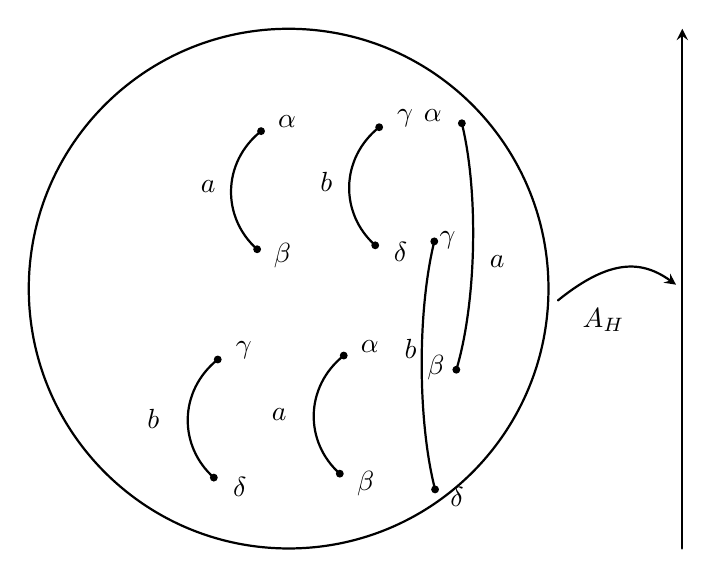
\begin{tikzpicture}[line cap=round,line join=round,>=stealth]
\draw[thick] (1.3,0) circle (3.3);
\fill (0.95,2.0) circle (0.05); \node at (1.28,2.12) {$\alpha$};
\draw[thick] (0.95,2.0) .. controls (0.45,1.6) and (0.45,0.9) .. (0.9,0.5);
\fill (0.9,0.5) circle (0.05); \node at (1.22,0.42) {$\beta$};
\node at (0.28,1.3) {$a$};
\fill (2.45,2.05) circle (0.05); \node at (2.78,2.17) {$\gamma$};
\draw[thick] (2.45,2.05) .. controls (1.95,1.65) and (1.95,0.95) .. (2.4,0.55);
\fill (2.4,0.55) circle (0.05); \node at (2.72,0.47) {$\delta$};
\node at (1.78,1.35) {$b$};
\fill (0.4,-0.9) circle (0.05); \node at (0.73,-0.78) {$\gamma$};
\draw[thick] (0.4,-0.9) .. controls (-0.1,-1.3) and (-0.1,-2.0) .. (0.35,-2.4);
\fill (0.35,-2.4) circle (0.05); \node at (0.68,-2.52) {$\delta$};
\node at (-0.42,-1.65) {$b$};
\fill (2.0,-0.85) circle (0.05); \node at (2.33,-0.73) {$\alpha$};
\draw[thick] (2.0,-0.85) .. controls (1.5,-1.25) and (1.5,-1.95) .. (1.95,-2.35);
\fill (1.95,-2.35) circle (0.05); \node at (2.28,-2.47) {$\beta$};
\node at (1.18,-1.6) {$a$};
\fill (3.5,2.1) circle (0.05); \node at (3.13,2.2) {$\alpha$};
\draw[thick] (3.5,2.1) .. controls (3.72,1.2) and (3.68,-0.2) .. (3.43,-1.03);
\fill (3.43,-1.03) circle (0.05); \node at (3.17,-1.0) {$\beta$};
\node at (3.95,0.35) {$a$};
\fill (3.15,0.6) circle (0.05); \node at (3.32,0.62) {$\gamma$};
\draw[thick] (3.15,0.6) .. controls (2.93,-0.3) and (2.94,-1.7) .. (3.16,-2.55);
\fill (3.16,-2.55) circle (0.05); \node at (3.44,-2.65) {$\delta$};
\node at (2.85,-0.77) {$b$};
\draw[thick,->] (6.3,-3.3) -- (6.3,3.3);
\node at (5.88,2.95) {$\RR$};
\draw[thick,->] (4.72,-0.15) .. controls (5.4,0.4) and (5.8,0.35) .. (6.22,0.05);
\node at (5.3,-0.4) {$\scr{A}_{H}$};
\end{tikzpicture}
\caption{}
\label{fig:action-ordering}
\end{figure}

\begin{proof}[\cref{thm:trajectories-action-ordering}的证明]
若 $(s_{n})$ 有一个有限的极限 $\sigma$，那么我们显然有 $a(s+\sigma,t)=b(s,t)$，从而 $\widehat{a}=\widehat{b}$。因此我们假定 $\lim s_{n}=+\infty$，并取定 $\sigma$、$\tau\in\RR$。对充分大的 $n$，我们有 $s_{n}+\sigma\ge\tau$。由于 $\scr{A}_{H}$ 沿 $\scr{M}$ 的诸\trTrajectory{}是递减的，于是我们有\footnote{译注：原书下式印作 $\scr{A}_{H}(\lambda_{n}(s_{n}+\sigma,\cdot)\le\scr{A}_{H}(\tau,\cdot))$；按取极限后的一式 $\scr{A}_{H}(b(\sigma,\cdot))\le\scr{A}_{H}(a(\tau,\cdot))$（其中 $\lambda_{n}(s_{n}+\sigma,\cdot)\to b(\sigma,\cdot)$、$\lambda_{n}(\tau,\cdot)\to a(\tau,\cdot)$），疑应在左端补上 $\lambda_{n}(\cdots)$ 的右括号、并在右端补出 $\lambda_{n}$（即 $\scr{A}_{H}(\lambda_{n}(s_{n}+\sigma,\cdot))\le\scr{A}_{H}(\lambda_{n}(\tau,\cdot))$），此处径改。——译者注}
\[
\scr{A}_{H}\bigl(\lambda_{n}(s_{n}+\sigma,\cdot)\bigr)\le\scr{A}_{H}\bigl(\lambda_{n}(\tau,\cdot)\bigr)\text{。}
\]
令 $n$ 趋于无穷，我们便得到
\[
\scr{A}_{H}\bigl(b(\sigma,\cdot)\bigr)\le\scr{A}_{H}\bigl(a(\tau,\cdot)\bigr)
\]
对 $\RR$ 中的一切 $\sigma$ 与 $\tau$ 都成立。令 $\sigma$ 趋于 $-\infty$、$\tau$ 趋于 $+\infty$，我们便发现
\[
\scr{A}_{H}(\beta)\ge\scr{A}_{H}(\gamma)\text{，}
\]
这就证明了这条引理（序列 $(s_{n})$ 趋于 $-\infty$ 的情形是类似的）。
\end{proof}

\begin{proof}[\cref{thm:lift-limit-critical}的证明]
现在我们把这条引理应用于序列 $\widetilde{\ell}_{n}$。由于 $\widetilde{\ell}_{n}\in\scr{M}(x,z)$，显然 $\lambda=\lim\widetilde{\ell}_{n}$ 满足\footnote{译注：原书此处印作 $\lambda=\lim\ell_{n}$；按\cref{thm:lift-limit-critical}的假设（$\widetilde{\ell}_{n}$ 在 $\scr{M}$ 中\trConvergence{}到 $\lambda$）以及本句开头的 $\widetilde{\ell}_{n}\in\scr{M}(x,z)$，疑漏一波浪号，应为 $\lambda=\lim\widetilde{\ell}_{n}$，此处径改。又，下文 $\lambda\notin\{\widehat{u},\widehat{v}\}$ 一句，按字面 $\lambda\in\scr{M}$ 与 $\widehat{u}$、$\widehat{v}\in\scr{L}$ 不同空间，疑应读作 $\lambda\notin\{\widetilde{u},\widetilde{v}\}$（或 $\widehat{\lambda}\notin\{\widehat{u},\widehat{v}\}$），此处照原书排印，存疑备案。——译者注}
\[
\scr{A}_{H}(x)\ge\scr{A}_{H}\bigl(\lambda(s,\cdot)\bigr)\ge\scr{A}_{H}(z)\qquad\text{对一切 } s\in\RR\text{。}
\]
若 $\lambda\notin\{\widehat{u},\widehat{v}\}$，那么由于 $\ell_{n}$ 趋于 $(\widehat{u},\widehat{v})$，前一条引理就蕴含
\[
\scr{A}_{H}(\lambda)\in\bigl\{\scr{A}_{H}(x),\scr{A}_{H}(y),\scr{A}_{H}(z)\bigr\}\text{。}
\]
特别地，$\scr{A}_{H}(\lambda(s,\cdot))$ 不依赖于 $s$，于是 $\lambda$ 是 $X_{t}$ 的一条\trPeriodic\trTrajectory。由于我们已经假定 $\scr{A}_{H}$ 的诸\trCriticalValue{}两两不同（\cref{thm:distinct-critical-values}），我们此刻便已证明了
\[
\lambda\in\{x,y,z\}\text{。}\qedhere
\]
\end{proof}

\begin{remark}\label{thm:broken-lift-limits}
用同样的证明，我们可以看到，更一般地，如果序列 $\ell_{n}\in\scr{L}(\alpha,\beta)$ 满足
\[
\lim_{n\to+\infty}\ell_{n}=(u_{1},\dots,u_{k})\in\overline{\scr{L}}(\alpha,\beta)\quad\text{其中 } u_{i}\in\scr{L}(\gamma_{i-1},\gamma_{i})\text{，}\ \gamma_{0}=\alpha\text{，}\gamma_{k}=\beta\text{，}
\]
那么，对 $\ell_{n}$ 的任一\trLift{} $\widetilde{\ell}_{n}$，若序列 $\widetilde{\ell}_{n}$ 是\trConvergence{}的，我们就有
\[
\lim_{n\to+\infty}\widetilde{\ell}_{n}\in\bigl\{\widehat{u}_{1},\dots,\widehat{u}_{k},\gamma_{0},\dots,\gamma_{k}\bigr\}\text{。}
\]
\end{remark}

这些预备工作就绪之后，让我们进入正题。

\begin{proof}[\cref{thm:lift-exp-decay}的证明]
我们取定一个实数 $\varepsilon>0$。下面这条引理的证明是显然的，它是\trManifold{} $W$ 的\trCompact{}性的一个直接推论。

\begin{lemma}\label{thm:exp-convex-ball}
存在 $\delta$ 与 $\delta'$，使得 $0<\delta<\delta'<\rho_{\mathrm{inj}}$，并且使得：对每个 $a\in W$ 与一切 $p,q\in B(a,\delta')$，我们可以写成
\[
q=\exp_{p}Y\text{，}\qquad\text{其中 } \|Y\|<\varepsilon\text{，}
\]
而且，对每个 $a\in W$、一切 $p,q\in B(a,\delta)$ 与一切 $\beta^{-},\beta^{+}\in[0,1]$，我们有
\[
\exp_{a}\bigl(\beta^{-}\exp_{a}^{-1}(p)+\beta^{+}\exp_{a}^{-1}(q)\bigr)\in B(a,\delta')\text{。}
\]
\noqed
\end{lemma}

我们选取 $\ell_{n}$ 的一个满足 $\scr{A}_{H}\bigl(\widetilde{\ell}_{n}(0,\cdot)\bigr)=\scr{A}_{H}(y)$ 的\trLift{} $\widetilde{\ell}_{n}$。序列 $\widetilde{\ell}_{n}$ 在 $\scr{M}$ 中是\trConvergence{}的（必要时抽取一个子序列之后），并且由\cref{thm:lift-limit-critical}，它的极限是 $y$。

让我们来证明 $\widetilde{\ell}_{n}$ 满足\cref{thm:lift-exp-decay}的诸结论。下面就是证明的想法。设 $w_{n}$ 表示 $u$ 与 $v$ 的一个\trPregluing，即 $w_{n}=w_{\nu,\rho_{n}}$，其中 $\nu\colon\RR_{+}\to\RR_{+}$ 是一个尚待确定的函数。我们取定一个 $\varepsilon>0$，并设 $B(x,\delta)$、$B(y,\delta)$、$B(z,\delta)$ 表示\footnote{我们回顾过：$B(y,\delta)=\bigl\{\chi\colon S^{1}\to W\mid d\bigl(\chi(t),y(t)\bigr)<\delta\ \forall t\in S^{1}\bigr\}$。}\trLoopSpace{} $\scr{L}W$ 上对于 $\cC^{0}$ 距离的开球（常数 $\delta$ 就是\cref{thm:exp-convex-ball}所给出的那个，并且我们可以——而且我们也确实如此——假定这些球两两不相交）。当 $s$ 非常小时，$\widetilde{\ell}_{n}(s,\cdot)$ 与 $w_{n}(s,\cdot)$ 落在 $B(x,\delta)$ 中；当 $s$ 靠近 $0$ 时，它们落在 $B(y,\delta)$ 中；而当 $s$ 非常大时，它们落在 $B(z,\delta)$ 中。在这三种情形里，我们都可以应用\cref{thm:exp-convex-ball}来结束证明。对其余的 $s$ 值，我们利用 $\ell_{n}$ 在 $\overline{\scr{L}}(x,z)$ 中趋于 $(\widehat{u},\widehat{v})$ 这一事实，它转化为：存在诸序列 $\sigma_{n}$ 与 $\tau_{n}$ 以及实数 $\sigma_{\star}$ 与 $\tau_{\star}$，使得
\[
\lim\widetilde{\ell}_{n}(s-\sigma_{n},t)=u(s+\sigma_{\star},t)\qquad\text{与}\qquad \lim\widetilde{\ell}_{n}(s+\tau_{n},t)=v(s+\tau_{\star},t)\text{。}
\]
这个\trConvergence{}在 $\RR\times S^{1}$ 的诸\trCompact{}子集上是一致的。第一个极限告诉我们：在 $(K-\sigma_{n})\times S^{1}$（其中 $K$ 是 $\RR$ 的一个\trCompact{}子集）上，$\widetilde{\ell}_{n}(s,t)$ 与 $u(s+\sigma_{n}+\sigma_{\star},t)$ 相接近。我们必须用这类开集去“\trCovering{}住”\cref{fig:pregluing-cover}中未打阴影的部分。

\begin{figure}[htbp]
\centering
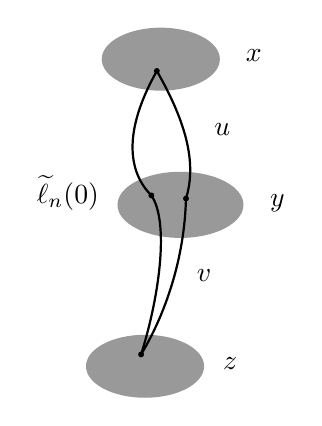
\begin{tikzpicture}[line cap=round,line join=round]
\fill[gray!80] (0.1,3.05) ellipse (0.75 and 0.4);
\node at (1.28,3.1) {$x$};
\fill[gray!80] (0.35,1.2) ellipse (0.8 and 0.42);
\node at (1.58,1.22) {$y$};
\fill[gray!80] (-0.1,-0.85) ellipse (0.75 and 0.4);
\node at (0.98,-0.82) {$z$};
\draw[thick] (0.05,2.9) .. controls (0.45,2.2) and (0.55,1.7) .. (0.42,1.28);
\node at (0.88,2.15) {$u$};
\draw[thick] (0.42,1.28) .. controls (0.4,0.5) and (0.15,-0.2) .. (-0.15,-0.7);
\node at (0.65,0.3) {$v$};
\draw[thick] (0.05,2.9) .. controls (-0.4,2.1) and (-0.3,1.6) .. (-0.02,1.32)
 .. controls (0.2,1.0) and (0.1,0.1) .. (-0.15,-0.7);
\draw[fill] (-0.02,1.32) circle (0.03);
\node at (-1.08,1.35) {$\widetilde{\ell}_{n}(0)$};
\draw[fill] (0.05,2.9) circle (0.03);
\draw[fill] (0.42,1.28) circle (0.03);
\draw[fill] (-0.15,-0.7) circle (0.03);
\end{tikzpicture}
\caption{}
\label{fig:pregluing-cover}
\end{figure}

诸序列 $\sigma_{n}$ 与 $\tau_{n}$ 的选取因此非常重要。这也正是将决定\trPregluing{} $w_{n}=w_{\nu,\rho_{n}}$ 之选取的东西。为了简化记号，我们在下文中省略变量 $t\in S^{1}$。我们已经看到，在 $\scr{M}$ 中 $y=\lim\widetilde{\ell}_{n}$，特别地，$\lim\widetilde{\ell}_{n}(0)=y$。于是，对 $n\ge N_{\varepsilon}$，我们有 $\widetilde{\ell}_{n}(0)\in B(y,\delta)$（仍然是 $\scr{L}W$ 上的 $\cC^{0}$ 距离）。我们令
\[
\sigma_{n}=\sup\bigl\{s>0\mid \widetilde{\ell}_{n}([-s,0])\subset B(y,\delta)\bigr\}
\]
与
\[
\tau_{n}=\sup\bigl\{s>0\mid \widetilde{\ell}_{n}([0,s])\subset B(y,\delta)\bigr\}\text{。}
\]
于是 $\widetilde{\ell}_{n}(-\sigma_{n})$ 与 $\widetilde{\ell}_{n}(\tau_{n})\in\partial\overline{B}(y,\delta)$。我们有：

（1）诸序列 $\sigma_{n}$ 与 $\tau_{n}$ 趋于 $+\infty$。的确，假如序列 $(\sigma_{n})$ 是\trBounded{}的，那么 $\widetilde{\ell}_{n}([-\sigma_{n},0])$ 就会趋于 $y$，从而我们就会有 $\lim\widetilde{\ell}_{n}(-\sigma_{n})=y$，而这是荒谬的。同样的推理也适用于 $\tau_{n}$。

（2）设 $\widetilde{\ell}^{1}_{n}(s)=\widetilde{\ell}_{n}(s-\sigma_{n})$，并设 $\widetilde{\ell}^{2}_{n}(s)=\widetilde{\ell}_{n}(s+\tau_{n})$。那么，在必要时抽取一个子序列之后，
\[
\lim\widetilde{\ell}^{1}_{n}(s)=u(s+\sigma_{\star})\quad\text{与}\quad \lim\widetilde{\ell}^{2}_{n}(s)=v(s+\tau_{\star})\qquad\text{于 } \scr{M}\text{ 中，}\ \sigma_{\star},\tau_{\star}\in\RR\text{。}
\]
的确，我们有 $\widetilde{\ell}^{1}_{n}(0)=\widetilde{\ell}_{n}(-\sigma_{n})\in\partial\overline{B}(y,\delta)$。因此，序列 $\widetilde{\ell}^{1}_{n}$ 不趋于 $y$。它也不趋于 $x$，因为 $\widetilde{\ell}^{1}_{n}(0)\in\partial\overline{B}(y,\delta)$，从而对任何 $n$，$\widetilde{\ell}^{1}_{n}(0)$ 都不在 $B(x,\delta)$ 之中。此外，
\[
\scr{A}_{H}\bigl(\widetilde{\ell}^{1}_{n}(0)\bigr)=\scr{A}_{H}\bigl(\widetilde{\ell}_{n}(-\sigma_{n})\bigr)>\scr{A}_{H}\bigl(\widetilde{\ell}_{n}(0)\bigr)=\scr{A}_{H}(y)\text{。}
\]
由\cref{thm:lift-limit-critical}，这就蕴含
\[
\lim\widetilde{\ell}^{1}_{n}(s)=u(s+\sigma_{\star})\qquad\text{于 } \scr{M}\text{ 中，对一个常数 } \sigma_{\star}\in\RR\text{。}
\]
类似地，我们有
\[
\lim\widetilde{\ell}^{2}_{n}(s)=v(s+\tau_{\star})\qquad\text{于 } \scr{M}\text{ 中，对一个常数 } \tau_{\star}\in\RR\text{。}
\]

现在让我们令
\[
\sigma'_{n}=\inf\bigl\{s>0\mid \widetilde{\ell}_{n}(]-\infty,-s])\subset B(x,\delta)\bigr\}
\]
与
\[
\tau'_{n}=\inf\bigl\{s>0\mid \widetilde{\ell}_{n}([s,+\infty[)\subset B(z,\delta)\bigr\}\text{，}
\]
从而显然有 $\widetilde{\ell}_{n}(-\sigma'_{n})\in\partial\overline{B}(x,\delta)$ 与 $\widetilde{\ell}_{n}(\tau'_{n})\in\partial\overline{B}(z,\delta)$。还要注意下面这一点：

（1）我们有 $\sigma'_{n}\ge\sigma_{n}$ 与 $\tau'_{n}\ge\tau_{n}$。特别地，诸序列 $\sigma'_{n}$ 与 $\tau'_{n}$ 趋于 $+\infty$。的确，假定 $\sigma_{n}>\sigma'_{n}$，并取一个 $\sigma\in[\sigma'_{n},\sigma_{n}]$。$\sigma'_{n}$ 与 $\sigma_{n}$ 的定义于是就蕴含 $\widetilde{\ell}_{n}(-\sigma)\in B(x,\delta)\cap B(y,\delta)$，而这是荒谬的，因为这两个球曾被假定是不相交的。同样的论证也适用于 $\tau_{n}$ 与 $\tau'_{n}$。

（2）在必要时抽取一个子序列之后，我们有
\[
\lim\widetilde{\ell}_{n}(s-\sigma'_{n})=u(s+\sigma'_{\star})\qquad\text{与}\qquad \lim\widetilde{\ell}_{n}(s+\tau'_{n})=v(s+\tau'_{\star})
\]
对一些常数 $\sigma'_{\star},\tau'_{\star}\in\RR$ 成立（这个\trConvergence{}是在 $\scr{M}$ 中的，也就是说，在 $\RR\times S^{1}$ 的诸\trCompact{}子集上是一致\trConvergence）。设 $\widetilde{\ell}^{3}_{n}(s)=\widetilde{\ell}_{n}(s-\sigma'_{n})$，我们有
\[
\widetilde{\ell}^{3}_{n}(0)\in\partial\overline{B}(x,\delta)\qquad\text{与}\qquad \scr{A}_{H}\bigl(\widetilde{\ell}^{3}_{n}(0)\bigr)\in\,]\scr{A}_{H}(y),\scr{A}_{H}(x)[\text{。}
\]
\cref{thm:lift-limit-critical}于是便像上面那样蕴含：$\widetilde{\ell}^{3}_{n}(s)$ \trConvergence{}到 $u(s+\sigma'_{\star})$。对 $\widetilde{\ell}^{4}_{n}=\widetilde{\ell}_{n}(s+\tau'_{n})$ 也有一个类似的论证。

我们将需要一条比这最后一条注记更强的结果，即下面这条。

\begin{lemma}\label{thm:sigma-prime-difference-bounded}
诸序列 $\sigma'_{n}-\sigma_{n}$ 与 $\tau'_{n}-\tau_{n}$ 是\trBounded{}的。
\end{lemma}

\begin{proof}
假定相反地 $\sigma'_{n}-\sigma_{n}$ 趋于 $+\infty$。我们将证明这会导出一个矛盾。由于 $\sigma'_{n}$ 与 $\sigma_{n}$ 都是正的，我们有
\[
\scr{A}_{H}\bigl(\widetilde{\ell}_{n}(-\sigma_{n})\bigr)\ \text{与}\ \scr{A}_{H}\bigl(\widetilde{\ell}_{n}(-\sigma'_{n})\bigr)\in\bigl[\scr{A}_{H}\bigl(\widetilde{\ell}_{n}(0)\bigr),\scr{A}_{H}(x)\bigr]\subset\bigl[\scr{A}_{H}(z),\scr{A}_{H}(x)\bigr]\text{。}
\]
我们将证明 $\scr{A}_{H}\bigl(\widetilde{\ell}_{n}(-\sigma'_{n})\bigr)-\scr{A}_{H}\bigl(\widetilde{\ell}_{n}(-\sigma_{n})\bigr)$ 趋于 $+\infty$。\footnote{译注：原书此处首项印作 $\scr{A}_{H}\bigl(\widetilde{\ell}_{n}(\sigma'_{n})\bigr)$；按紧随其后的积分等式，其左端即 $\scr{A}_{H}(\widetilde{\ell}_{n}(-\sigma'_{n}))-\scr{A}_{H}(\widetilde{\ell}_{n}(-\sigma_{n}))$，疑漏一枚负号，应为 $\scr{A}_{H}\bigl(\widetilde{\ell}_{n}(-\sigma'_{n})\bigr)$，此处径改。——译者注}我们有
\[
\begin{aligned}
\scr{A}_{H}\bigl(\widetilde{\ell}_{n}(-\sigma'_{n})\bigr)-\scr{A}_{H}\bigl(\widetilde{\ell}_{n}(-\sigma_{n})\bigr)&=\int_{-\sigma_{n}}^{-\sigma'_{n}}\frac{\partial}{\partial s}\scr{A}_{H}\bigl(\widetilde{\ell}_{n}(s)\bigr)\,ds\\[4pt]
&=\int_{-\sigma'_{n}}^{-\sigma_{n}}\int_{S^{1}}\Bigl\|\frac{\partial\widetilde{\ell}_{n}}{\partial s}(s,t)\Bigr\|^{2}\,dt\,ds
\end{aligned}
\]
（该范数就是由 $W$ 上的\trMetric{}所定义的那个）。于是存在一些 $c_{n}\in[-\sigma'_{n},-\sigma_{n}]$，使得
\[
\int_{S^{1}}\Bigl\|\frac{\partial\widetilde{\ell}_{n}}{\partial s}(c_{n},t)\Bigr\|^{2}\,dt\quad\text{趋于 } 0\text{，}
\]
因为若不然，在必要时抽取一个子序列之后，我们就会有\footnote{译注：原书此处区间印作 $[-\sigma'_{n},\sigma_{n}]$；矛盾论证正需在上述积分的区间上逐点控制被积函数（上文 $c_{n}$ 亦恰取自 $[-\sigma'_{n},-\sigma_{n}]$），疑末端 $\sigma_{n}$ 漏一枚负号，应为 $[-\sigma'_{n},-\sigma_{n}]$。又，上文\trEnergy{}差等式第二行的重积分，其积分限原书亦印作自 $-\sigma_{n}$ 到 $-\sigma'_{n}$ 的反向——左端系沿解作用递减所得的正\trEnergy{}差，而以反向积分限积非负被积函数其值非正，二者相抵——正确应自 $-\sigma'_{n}$ 积到 $-\sigma_{n}$。此处均径改。——译者注}
\[
\int_{S^{1}}\Bigl\|\frac{\partial\widetilde{\ell}_{n}}{\partial s}(s,t)\Bigr\|^{2}\,dt\ge\gamma_{0}\qquad\text{对 } s\in[-\sigma'_{n},-\sigma_{n}]\text{，}
\]
从而
\[
\int_{-\sigma'_{n}}^{-\sigma_{n}}\int_{S^{1}}\Bigl\|\frac{\partial\widetilde{\ell}_{n}}{\partial s}(s,t)\Bigr\|^{2}\,dt\,ds\ge\gamma_{0}(\sigma'_{n}-\sigma_{n})\qquad\text{趋于 } +\infty\text{，}
\]
这与上面所述的包含关系相矛盾。\footnote{译注：原书此式下界印作 $\gamma_{0}^{2}(\sigma'_{n}-\sigma_{n})$；按上一式的逐点下界为 $\gamma_{0}$，且稍后式中的余量亦作 $\gamma_{0}$，疑平方为衍字，应为 $\gamma_{0}(\sigma'_{n}-\sigma_{n})$，此处径改。——译者注}由于 $\widetilde{\ell}_{n}$ 是\trFloerEquation{}的一个解，我们也可以把这写成
\[
\int_{S^{1}}\Bigl\|\frac{\partial\widetilde{\ell}_{n}}{\partial t}(c_{n},t)-X_{t}\bigl(\widetilde{\ell}_{n}(c_{n},t)\bigr)\Bigr\|^{2}\,dt\qquad\text{趋于 } 0\text{。}
\]
设 $\widetilde{\ell}^{5}_{n}(s)=\widetilde{\ell}_{n}(s+c_{n})$。由于 $c_{n}\in[-\sigma'_{n},-\sigma_{n}]$，我们有
\[
\scr{A}_{H}\bigl(\widetilde{\ell}^{5}_{n}(0)\bigr)=\scr{A}_{H}\bigl(\widetilde{\ell}_{n}(c_{n})\bigr)\in\bigl[\scr{A}_{H}\bigl(\widetilde{\ell}_{n}(-\sigma_{n})\bigr),\ \scr{A}_{H}\bigl(\widetilde{\ell}_{n}(-\sigma'_{n})\bigr)\bigr]\text{。}
\]
其次，由于
\[
\lim_{n\to+\infty}\scr{A}_{H}\bigl(\widetilde{\ell}_{n}(-\sigma_{n})\bigr)=\lim\scr{A}_{H}\bigl(\widetilde{\ell}^{1}_{n}(0)\bigr)=\scr{A}_{H}\bigl(u(\sigma_{\star})\bigr)
\]
与
\[
\lim\scr{A}_{H}\bigl(\widetilde{\ell}_{n}(-\sigma'_{n})\bigr)=\scr{A}_{H}\bigl(u(\sigma'_{\star})\bigr)\text{，}
\]
我们便推出：对某个 $\gamma_{0}>0$ 与每个 $n$，
\[
\scr{A}_{H}\bigl(\widetilde{\ell}^{5}_{n}(0)\bigr)\in\,]\scr{A}_{H}(y)+\gamma_{0},\ \scr{A}_{H}(x)-\gamma_{0}[\text{。}
\]
应用\cref{thm:lift-limit-critical}，我们于是发现 $\widetilde{\ell}^{5}_{n}(s)$ 在 $\scr{M}$ 中趋于 $u(s+c_{\star})$，特别地，$\widetilde{\ell}_{n}(c_{n})=\widetilde{\ell}^{5}_{n}(0)$ 对于 $S^{1}$ 上的 $\cC^{\infty}$ \trTopology{}一致\trConvergence{}到 $u(c_{\star})$。结合上面给出的关系式，这就给出
\[
\int_{S^{1}}\Bigl\|\frac{\partial u}{\partial t}(c_{\star},t)-X_{t}\bigl(u(c_{\star},t)\bigr)\Bigr\|^{2}\,dt=0
\]
从而
\[
\frac{\partial u}{\partial t}(c_{\star},t)-X_{t}\bigl(u(c_{\star},t)\bigr)=0\text{，}
\]
这意味着 $u(c_{\star})$ 是 $\scr{A}_{H}$ 的一个\trCriticalPoint。我们把这个\trCriticalPoint{}称作 $\alpha$。对每个 $t\in S^{1}$，我们有
\[
\begin{aligned}
\frac{\partial u}{\partial s}(c_{\star},t)&=-J\bigl(u(c_{\star},t)\bigr)\Bigl(\frac{\partial u}{\partial t}(c_{\star},t)-X_{t}\bigl(u(c_{\star},t)\bigr)\Bigr)\\[4pt]
&=-J(\alpha)\Bigl(\frac{\partial u}{\partial t}(\alpha)-X_{t}(\alpha)\Bigr)=0\text{。}
\end{aligned}
\]
从而，\trCriticalPoint{}集 $C(u)$ 包含 $c_{\star}\times S^{1}$，这就与“由\cref{thm:critical-points-discrete}，这个集合是离散的”这一事实相矛盾。

我们得出结论：序列 $\sigma'_{n}-\sigma_{n}$ 是\trBounded{}的。我们可以用同样的方法证明 $\tau'_{n}-\tau_{n}$ 也是\trBounded{}的，这就结束了\cref{thm:sigma-prime-difference-bounded}的证明。
\end{proof}

让我们来完成\cref{thm:lift-exp-decay}的证明。设 $A$、$B$ 与 $C\in\RR$ 是使得下列条件成立的常数：

\begin{itemize}
\item 对 $s\le A$，$u(s)\in B(x,\delta)$ 且 $v(s)\in B(y,\delta)$；
\item 对 $s\ge B$，$u(s)\in B(y,\delta)$ 且 $v(s)\in B(z,\delta)$；
\item $\sigma'_{n}-\sigma_{n}\le C$ 且 $\tau'_{n}-\tau_{n}\le C$（$C>0$）。
\end{itemize}

这个 $\delta$ 就是\cref{thm:exp-convex-ball}所给出的那个，其中的 $\varepsilon>0$ 仍然是取定的。我们还要用在 $\sigma_{n}$ 与 $\tau_{n}$ 的定义之后的第二条注记中所定义的诸常数 $\sigma_{\star}$、$\tau_{\star}$，并考虑一个\trCompact{}区间 $[E,F]$，使得：

\begin{itemize}
\item $E<0$，$E+\sigma_{\star}\le A$，$E+\tau_{\star}\le A$；
\item $F>0$，$F+\sigma_{\star}\ge B$，$F+\tau_{\star}\ge B$；
\item 对每个 $n\in\NN$，$\sigma'_{n}-\sigma_{n}\le -E$ 且 $\tau'_{n}-\tau_{n}\le F$。
\end{itemize}

我们知道，$\widetilde{\ell}_{n}(s-\sigma_{n})$ 在 $\RR\times S^{1}$ 的诸\trCompact{}子集上一致\trConvergence{}到 $u(s+\sigma_{\star})$。于是，对一个取定的 $\varepsilon>0$，存在一个 $N_{\varepsilon}$，使得对 $n\ge N_{\varepsilon}$、$t\in S^{1}$ 与 $s\in[E,F]$，我们有
\[
\widetilde{\ell}_{n}(s-\sigma_{n},t)=\exp_{u(s+\sigma_{\star},t)}Y^{1}_{n}(s,t)\qquad\text{其中 } \bigl\|Y^{1}_{n}(s,t)\bigr\|\le\varepsilon
\]
（相对于\trEuclidean{}范数）。把 $s$ 换成 $s+\sigma_{n}$，我们便发现：对 $n\ge N_{\varepsilon}$，
\[
\widetilde{\ell}_{n}(s,t)=\exp_{u(s+\sigma_{n}+\sigma_{\star},t)}Y_{n}(s,t)
\]
其中
\[
\|Y_{n}(s,t)\|\le\varepsilon\qquad\text{对每个 } (s,t)\in[E-\sigma_{n},F-\sigma_{n}]\times S^{1}\text{。}
\]
以同样的方式，对 $n\ge N_{\varepsilon}$，我们有
\[
\widetilde{\ell}_{n}(s,t)=\exp_{v(s+\tau_{\star}-\tau_{n},t)}Y_{n}(s,t)
\]
其中
\[
\|Y_{n}(s,t)\|\le\varepsilon\qquad\text{对每个 } (s,t)\in[E+\tau_{n},F+\tau_{n}]\times S^{1}\text{。}
\]
我们回顾过：对充分大的 $n$，区间 $[E-\sigma_{n},F-\sigma_{n}]$ 与 $[E+\tau_{n},F+\tau_{n}]$ 是不相交的……因此，由这两条关系式所定义的两个 $Y_{n}$ 之间不会产生任何混淆。

我们如下定义一个\trPregluing{} $w_{n}(s,t)$：
\[
w_{n}(s,t)=
\left\{
\begin{array}{ll}
u(s+\sigma_{\star}+\sigma_{n},t) & \text{若 } s\le -1\text{，}\\[10pt]
\begin{aligned}
\exp_{y(t)}\Bigl(\beta^{-}(s)\exp_{y(t)}^{-1}u(s+\sigma_{\star}+\sigma_{n},t)\\
+\ \beta^{+}(s)\exp_{y(t)}^{-1}v(s+\tau_{\star}-\tau_{n},t)\Bigr)
\end{aligned}
& \text{若 } s\in[-1,1]\text{，}\\[10pt]
v(s+\tau_{\star}-\tau_{n},t) & \text{若 } s\ge 1\text{。}
\end{array}
\right.
\]

让我们来证明：对每个 $n\ge N_{\varepsilon}$ 与 $(s,t)\in\RR\times S^{1}$，我们有
\[
\widetilde{\ell}_{n}(s,t)=\exp_{w_{n}(s,t)}Y_{n}(s,t)\text{，}\qquad\text{其中 } \|Y_{n}(s,t)\|\le\varepsilon\text{。}
\]
为此，我们把 $\RR$ 切成几个区间：

（1）对 $s<E-\sigma_{n}\le-\sigma'_{n}$，我们有 $\widetilde{\ell}_{n}(s,t)\in B(x(t),\delta)$（由 $\sigma'_{n}$ 的定义），并且
\[
w_{n}(s,t)=u(s+\sigma_{\star}+\sigma_{n},t)\in B(x(t),\delta)
\]
因为
\[
s+\sigma_{\star}+\sigma_{n}\le E+\sigma_{\star}\le A\text{。}
\]
我们通过应用\cref{thm:exp-convex-ball}的第一条断言而得到所需要的关系式。

（2）对 $s\in[E-\sigma_{n},F-\sigma_{n}]$，利用 $Y_{n}$ 的定义便得到结果。

（3）对 $s\in[F-\sigma_{n},E+\tau_{n}]$，由 $\sigma_{n}$ 与 $\tau_{n}$ 的定义（利用不等式 $F>0$ 与 $E<0$），我们有 $\widetilde{\ell}_{n}(s)\in B(y,\delta)$。其次，$u(s+\sigma_{\star}+\sigma_{n})\in B(y,\delta)$，因为 $s+\sigma_{\star}+\sigma_{n}\ge B$；同样地，$v(s+\tau_{\star}-\tau_{n})\in B(y,\delta)$，因为 $s+\tau_{\star}-\tau_{n}\le E+\tau_{\star}\le A$。\cref{thm:exp-convex-ball}的第二条断言给出 $w_{n}(s,t)\in B(y(t),\delta')$；于是我们可以再一次应用它的第一条断言来得到所需要的关系式。

（4）$s\in[E+\tau_{n},F+\tau_{n}]$ 的情形与 $s\in[E-\sigma_{n},F-\sigma_{n}]$ 的情形类似。

（5）对 $s\ge F+\tau_{n}\ge\tau'_{n}$，由 $\tau'_{n}$ 的定义我们有 $\widetilde{\ell}_{n}(s)\in B(z,\delta)$，并且 $w_{n}(s,t)\in B(z(t),\delta)$，因为 $w_{n}(s,t)=v(s+\tau_{\star}-\tau_{n},t)$ 且 $s+\tau_{\star}-\tau_{n}\ge F+\tau_{\star}\ge B$。

我们于是对每个 $s\in\RR$ 都得到了所需要的关系式。注意，如果我们选取 $\varepsilon$ 充分小，那么可以假定：对每个 $n\ge N_{\varepsilon}$ 与 $(s,t)\in\RR\times S^{1}$，都有 $\|Y_{n}(s,t)\|_{W}<\rho_{\mathrm{inj}}$（即 $Y_{n}$ 对于 $W$ 上的\trMetric{}的范数），从而
\[
Y_{n}(s,t)=\exp_{w_{n}(s,t)}^{-1}\widetilde{\ell}_{n}(s,t)\qquad\text{为 } \cC^{\infty}\text{ 类的。}
\]

\cref{thm:lift-exp-decay}的证明几乎要完成了。令 $\rho_{n}=\sigma_{n}+\sigma_{\star}$，并设 $\nu$ 是一个满足 $\nu(\rho_{n})=\tau_{n}-\tau_{\star}$ 的 $\cC^{\infty}$ 类函数。我们可以——而且我们也确实如此——选取 $\nu$ 为一个递增函数（必要时再一次抽取诸序列 $\rho_{n}$ 与 $\tau_{n}$ 的子序列），它在 $\rho$ 趋于 $+\infty$ 时趋于 $+\infty$。于是，对 $n\ge N_{\varepsilon}$ 与 $(s,t)\in\RR\times S^{1}$，我们有
\[
\widetilde{\ell}_{n}(s,t)=\exp_{w_{\nu,\rho_{n}}(s,t)}Y_{n}(s,t)\qquad\text{其中 } \|Y_{n}(s,t)\|\le\varepsilon\text{，}
\]
而这一次，这个命题的证明就真正结束了。
\end{proof}

\subsection{第 3 步：命题 9.6.4 的证明}
\label{subsec:step3-proof-964}

我们现在要证明：由\cref{thm:lift-exp-decay}给出的 $Y_{n}$ 属于 $W^{1,p}(\RR\times S^{1};\RR^{m})$，其中 $p>2$。为此，我们将利用\trFloerEquation{}诸解的\trExponentialDecay{}（\cref{sec:exponential-decay}），也就是说下面这一事实：若 $\ell\in\scr{M}$，那么存在一个常数 $C>0$，使得对每个 $(s,t)\in\RR\times S^{1}$，我们有
\[
\Bigl\|\frac{\partial\ell}{\partial s}(s,t)\Bigr\|\le Ce^{-\delta|s|}
\]
（既可以用 $W$ 的\trMetric{}的范数，也可以用 $\RR^{m}$ 中的\trEuclidean{}范数；我们选取后者）。前一步给了我们关系式
\[
\widetilde{\ell}_{n}(s,t)=\exp_{w_{n}(s,t)}Y_{n}(s,t)\qquad\text{或者}\qquad Y_{n}(s,t)=\exp_{w_{n}(s,t)}^{-1}\widetilde{\ell}_{n}(s,t)\text{。}
\]
映射 $w_{n}$ 与 $\widetilde{\ell}_{n}$ 都具有\trExponentialDecay（$w_{n}$ 在 $|s|\ge1$ 时是\trFloerEquation{}的一个解），当我们证明下面这条引理时，这将会有用。

\begin{lemma}\label{thm:yn-exp-decay}
存在一个常数 $K>0$（一般依赖于 $n$），使得对每个 $(s,t)\in\RR\times S^{1}$，我们有
\[
\max\Bigl(\Bigl\|\frac{\partial Y_{n}}{\partial s}(s,t)\Bigr\|,\ \|Y_{n}(s,t)\|,\ \Bigl\|\frac{\partial Y_{n}}{\partial t}(s,t)\Bigr\|\Bigr)\le Ke^{-\delta|s|}\text{。}
\]
\end{lemma}

显然，这条引理立即蕴含\cref{thm:yn-w1p}的第一条断言。因此让我们来证明它。

\begin{proof}[\cref{thm:yn-exp-decay}的证明]
考虑 $W\times W$ 的开子集 $\Omega$：
\[
\Omega=\bigl\{(a,b)\in W\times W\mid d(a,b)<\rho_{\mathrm{inj}}\bigr\}\text{。}
\]
设 $\Phi\colon\Omega\to\RR^{m}$ 为如下定义的映射：
\[
\Phi(a,b)=\exp_{a}^{-1}(b)\in T_{a}W\subset\RR^{m}\text{。}
\]
设 $\Omega_{0}\subset\Omega$ 为
\[
\Omega_{0}=\bigl\{(a,b)\in W\times W\mid d(a,b)\le\rho_{\mathrm{inj}}/2\bigr\}\text{；}
\]
这是 $W\times W$ 的一个\trCompact{}子集。我们选取一个常数 $A<0$，使得对每个 $s\le A$ 与每个 $t\in S^{1}$，我们有
\[
\bigl(w_{n}(s,t),\widetilde{\ell}_{n}(s,t)\bigr)\in\Omega_{0}
\]
（我们可以验证：对 $s\le A$，$d\bigl(w_{n}(s,\cdot),x\bigr)\le\rho_{\mathrm{inj}}/6$ 且 $d\bigl(\widetilde{\ell}_{n}(s,\cdot),x\bigr)\le\rho_{\mathrm{inj}}/6$）。于是我们有
\[
Y_{n}(s,t)=\Phi\bigl(w_{n}(s,t),\widetilde{\ell}_{n}(s,t)\bigr)\qquad\text{对 } (s,t)\in\,]-\infty,A]\times S^{1}\text{。}
\]
由 $\Omega_{0}$ 的\trCompact{}性，存在一个 $M>0$，使得
\[
\bigl\|D_{(a,b)}\Phi\bigr\|\le M\qquad\forall(a,b)\in\Omega_{0}\text{。}
\]
从而对每个 $s\le A$ 与每个 $t\in S^{1}$，我们有
\[
\begin{aligned}
\Bigl\|\frac{\partial Y_{n}}{\partial s}(s,t)\Bigr\|&=\Bigl\|\frac{\partial}{\partial s}\Phi\bigl(w_{n}(s,t),\widetilde{\ell}_{n}(s,t)\bigr)\Bigr\|\\
&\le\Bigl\|D_{1}\Phi_{(w_{n}(s,t),\widetilde{\ell}_{n}(s,t))}\frac{\partial w_{n}}{\partial s}(s,t)\Bigr\|+\Bigl\|D_{2}\Phi_{(w_{n}(s,t),\widetilde{\ell}_{n}(s,t))}\frac{\partial\widetilde{\ell}_{n}}{\partial s}(s,t)\Bigr\|\\
&\le M\Bigl\|\frac{\partial w_{n}}{\partial s}(s,t)\Bigr\|+M\Bigl\|\frac{\partial\widetilde{\ell}_{n}}{\partial s}(s,t)\Bigr\|\\
&\le 2MCe^{\delta s}
\end{aligned}
\]
（由于\trExponentialDecay）。同样地，我们可以证明：对 $s\ge B$，
\[
\Bigl\|\frac{\partial Y_{n}}{\partial s}(s,t)\Bigr\|\le 2MCe^{-\delta s}\text{，}
\]
这就给出了引理中“对于 $\partial Y_{n}/\partial s$”的部分。现在让我们对 $Y_{n}$ 本身证明它。像前面一样取 $A<0$。对 $s_{1}\le s_{2}\le A<0$ 与 $t\in S^{1}$，我们有\footnote{译注：原书此处与下文 $\Gamma$ 的估计处（原书 p.351）分别印作 $\int_{s_{1}}^{s_{2}}Ke^{\delta s}\,ds=K\bigl(e^{\delta s_{2}}-e^{\delta s_{1}}\bigr)$ 与 $MC\int_{s_{1}}^{s_{2}}e^{\delta s}\,ds=MC\bigl(e^{\delta s_{2}}-e^{\delta s_{1}}\bigr)$，等号右端均漏因子 $1/\delta$（$\delta>0$）：应为 $\frac{K}{\delta}\bigl(e^{\delta s_{2}}-e^{\delta s_{1}}\bigr)$ 与 $\frac{MC}{\delta}\bigl(e^{\delta s_{2}}-e^{\delta s_{1}}\bigr)$。两处照原书排印，存疑备案；后续估计只消把 $\frac{1}{\delta}$ 并入常数（更名后仍记作 $K$、$MC$）即恢复原状，估计与结论均不受影响。——译者注}
\[
\begin{aligned}
\|Y_{n}(s_{2},t)-Y_{n}(s_{1},t)\|&=\Bigl\|\int_{s_{1}}^{s_{2}}\frac{\partial Y_{n}}{\partial s}(s,t)\,ds\Bigr\|\le\int_{s_{1}}^{s_{2}}\Bigl\|\frac{\partial Y_{n}}{\partial s}(s,t)\Bigr\|\,ds\\
&\le\int_{s_{1}}^{s_{2}}Ke^{\delta s}\,ds=K\bigl(e^{\delta s_{2}}-e^{\delta s_{1}}\bigr)\text{。}
\end{aligned}
\]
我们让 $s_{1}$ 在这个不等式中趋于 $-\infty$，并利用 $Y_{n}$ 作为 $\widetilde{\ell}_{n}$ 的函数的表达式，便得到
\[
\begin{aligned}
\lim_{s\to-\infty}Y_{n}(s,t)&=\lim_{s\to-\infty}\Phi\bigl(w_{n}(s,t),\widetilde{\ell}_{n}(s,t)\bigr)\\
&=\Phi\bigl(x(t),x(t)\bigr)=\exp_{x(t)}^{-1}x(t)=0\text{。}
\end{aligned}
\]
于是我们有
\[
\|Y_{n}(s_{2},t)\|\le Ke^{\delta s_{2}}\text{。}
\]
对 $s\ge B$ 如法炮制，便给出关于 $Y_{n}$ 的所希望的结果。为了结束\cref{thm:yn-exp-decay}的证明，我们还须对 $\partial Y_{n}/\partial t$ 证明一个同类型的不等式。

从 $Y_{n}$ 作为 $\widetilde{\ell}_{n}$ 的函数的表达式出发，我们发现
\[
\frac{\partial Y_{n}}{\partial t}(s,t)=D_{1}\Phi_{(w_{n}(s,t),\widetilde{\ell}_{n}(s,t))}\frac{\partial w_{n}}{\partial t}(s,t)+D_{2}\Phi_{(w_{n}(s,t),\widetilde{\ell}_{n}(s,t))}\frac{\partial\widetilde{\ell}_{n}}{\partial t}(s,t)\text{。}
\]
上面选取的负常数 $A$ 被假定小于 $-1$。对 $s\le A\le-1$，$w_{n}$ 是\trFloerEquation{}的一个解。于是在每个点 $(s,t)$ 处，我们都可以写成\footnote{译注：原书此处两括号内分别印作 $X_{t}(w_{n})-J(w_{n})\cdot\frac{\partial w_{n}}{\partial s}$ 与 $X_{t}(\widetilde{\ell}_{n})-J(\widetilde{\ell}_{n})\cdot\frac{\partial\widetilde{\ell}_{n}}{\partial s}$；按\trFloerEquation{} $\scr{F}(w)=0$（乘 $-J$ 解出 $\frac{\partial w}{\partial t}$）应得 $\frac{\partial w}{\partial t}=X_{t}(w)+J(w)\cdot\frac{\partial w}{\partial s}$，两括号内均应为正号。随后把括号拆成 $J\frac{\partial w}{\partial s}$ 与 $X_{t}$ 两部分分别取范数的估计不受此正负号影响，照原书排印，存疑备案。——译者注}
\[
\frac{\partial Y_{n}}{\partial t}=D_{1}\Phi_{(w_{n},\widetilde{\ell}_{n})}\Bigl(X_{t}(w_{n})-J(w_{n})\cdot\frac{\partial w_{n}}{\partial s}\Bigr)
+D_{2}\Phi_{(w_{n},\widetilde{\ell}_{n})}\Bigl(X_{t}(\widetilde{\ell}_{n})-J(\widetilde{\ell}_{n})\cdot\frac{\partial\widetilde{\ell}_{n}}{\partial s}\Bigr)
\]
（为了简化记号，我们省去了点 $(s,t)$），而对每个点 $(s,t)\in\,]-\infty,A]\times S^{1}$，我们可以写成
\[
\begin{aligned}
\Bigl\|\frac{\partial Y_{n}}{\partial t}\Bigr\|&\le\Bigl\|D_{1}\Phi_{(w_{n},\widetilde{\ell}_{n})}J(w_{n})\frac{\partial w_{n}}{\partial s}\Bigr\|+\Bigl\|D_{2}\Phi_{(w_{n},\widetilde{\ell}_{n})}J(\widetilde{\ell}_{n})\frac{\partial\widetilde{\ell}_{n}}{\partial s}\Bigr\|\\
&\quad+\bigl\|D_{1}\Phi_{(w_{n},\widetilde{\ell}_{n})}X_{t}(w_{n})+D_{2}\Phi_{(w_{n},\widetilde{\ell}_{n})}X_{t}(\widetilde{\ell}_{n})\bigr\|\text{，}
\end{aligned}
\]
从而
\[
\Bigl\|\frac{\partial Y_{n}}{\partial t}\Bigr\|\le Ke^{\delta s}+\bigl\|D_{1}\Phi_{(w_{n},\widetilde{\ell}_{n})}X_{t}(w_{n})+D_{2}\Phi_{(w_{n},\widetilde{\ell}_{n})}X_{t}(\widetilde{\ell}_{n})\bigr\|\text{。}
\]
在这最后一个不等式中，我们利用了范数 $\|D\Phi\|$ 与 $\|J\|$ 分别在 $\Omega_{0}$ 上与在 $W$ 上是一致\trBounded{}的这一事实，以及 $w_{n}$ 与 $\widetilde{\ell}_{n}$ 的\trExponentialDecay。为了给出最后一项的一个上界，考虑映射 $\Gamma\colon\Omega\to\RR^{m}$，其定义为
\[
\Gamma(a,b)=D_{1}\Phi(a,b)X_{t}(a)+D_{2}\Phi_{(a,b)}X_{t}(b)\text{，}
\]
于是我们想要估计的项就是 $\|\Gamma(w_{n}(s,t),\widetilde{\ell}_{n}(s,t))\|$。如上面那样，由\trCompact{}性，存在一个 $M>0$，使得对每个 $(a,b)\in\Omega_{0}$，都有 $\|D\Gamma_{(a,b)}\|\le M$。从而，对 $s_{1}\le s_{2}\le A$ 与 $t\in S^{1}$，我们有
\[
\begin{aligned}
&\bigl\|\Gamma(w_{n}(s_{2},t),\widetilde{\ell}_{n}(s_{2},t))-\Gamma(w_{n}(s_{1},t),\widetilde{\ell}_{n}(s_{1},t))\bigr\|\\
&\qquad\le\Bigl\|\int_{s_{1}}^{s_{2}}\frac{\partial}{\partial s}\Gamma\bigl(w_{n}(s,t),\widetilde{\ell}_{n}(s,t)\bigr)\,ds\Bigr\|\\
&\qquad\le\int_{s_{1}}^{s_{2}}\Bigl\|\frac{\partial}{\partial s}\Gamma\bigl(w_{n}(s,t),\widetilde{\ell}_{n}(s,t)\bigr)\Bigr\|\,ds\\
&\qquad=\int_{s_{1}}^{s_{2}}\Bigl\|D_{1}\Gamma_{(w_{n},\widetilde{\ell}_{n})}\frac{\partial w_{n}}{\partial s}+D_{2}\Gamma_{(w_{n},\widetilde{\ell}_{n})}\frac{\partial\widetilde{\ell}_{n}}{\partial s}\Bigr\|\,ds\\
&\qquad\le\int_{s_{1}}^{s_{2}}M\Bigl(\Bigl\|\frac{\partial w_{n}}{\partial s}\Bigr\|+\Bigl\|\frac{\partial\widetilde{\ell}_{n}}{\partial s}\Bigr\|\Bigr)\,ds\\
&\qquad\le MC\int_{s_{1}}^{s_{2}}e^{\delta s}\,ds=MC\bigl(e^{\delta s_{2}}-e^{\delta s_{1}}\bigr)\text{，}
\end{aligned}
\]
仍然利用\trExponentialDecay。\footnote{译注：原书此链首行第二项印作 $\Gamma(w_{n}(s,t),\widetilde{\ell}_{n}(s,t))$；按积分自变量跑遍整个 $[s_{1},s_{2}]$ 的语境，疑应为 $\Gamma(w_{n}(s_{1},t),\widetilde{\ell}_{n}(s_{1},t))$，此处径改。——译者注}令 $s_{1}$ 趋于 $-\infty$。我们有
\[
\begin{aligned}
\lim_{s\to-\infty}\Gamma\bigl(w_{n}(s,t),\widetilde{\ell}_{n}(s,t)\bigr)&=\Gamma\bigl(x(t),x(t)\bigr)\\
&=D_{1}\Phi_{(x(t),x(t))}X_{t}\bigl(x(t)\bigr)+D_{2}\Phi_{(x(t),x(t))}X_{t}\bigl(x(t)\bigr)\\
&=D_{1}\Phi_{(x(t),x(t))}x'(t)+D_{2}\Phi_{(x(t),x(t))}x'(t)
\end{aligned}
\]
因为 $x(t)$ 是\trVectorField{} $X_{t}$ 的一条\trTrajectory。我们发现
\[
\lim_{s\to-\infty}\Gamma\bigl(w_{n}(s,t),\widetilde{\ell}_{n}(s,t)\bigr)=\frac{\partial}{\partial t}\Phi\bigl(x(t),x(t)\bigr)=\frac{\partial}{\partial t}0=0\text{。}
\]
从而对 $s_{2}\le A$ 与 $t\in S^{1}$，我们有
\[
\bigl\|\Gamma\bigl(w_{n}(s_{2},t),\widetilde{\ell}_{n}(s_{2},t)\bigr)\bigr\|\le Ke^{\delta s_{2}}\text{。}
\]
我们以同样的方式处理 $s\ge B$ 的情形，以此结束\cref{thm:yn-exp-decay}的证明。
\end{proof}

正如我们已经指出过的，我们的 $Y_{n}$ 属于 $W^{1,p}(\RR\times S^{1};\RR^{m})$（对每个 $p>2$）这一事实便立即随之而来。为了结束\cref{thm:yn-w1p}的证明，我们还须证明：$Y_{n}$ 对于 $W^{1,p}$ 范数趋于 $0$。于是我们考虑沿\trPregluing{} $w_{n}$ 的一个酉\trTrivialization{} $(Z^{n}_{i})_{i}$，它像在\cref{sec:construction-psi-rho}中那样选取（参见\cref{fig:trivializations-w-rho}）。利用\trFrame{} $Z_{i}$，我们把 $Y_{n}$ 写成 $Y_{n}=i(\zeta_{n})$，其中 $\zeta_{n}\in W^{1,p}(\RR\times S^{1};\RR^{2n})$。这里的 $\scr{F}$ 表示\trFloer{}算子
\[
\scr{F}=\frac{\partial}{\partial s}+J\frac{\partial}{\partial t}+\operatorname{grad}(H_{t})\text{。}
\]
算子 $F\colon W^{1,p}(\RR\times S^{1};\RR^{2n})\to L^{p}(\RR\times S^{1};\RR^{2n})$ 由
\[
F(\zeta)=p\bigl(i(\zeta),\widetilde{\scr{F}}(i(\zeta))\bigr)
\]
所定义，其中
\[
\widetilde{\scr{F}}\colon W^{1,p}(\RR\times S^{1};\RR^{m})\longrightarrow L^{p}(\RR\times S^{1};\RR^{m})
\]
由
\[
\widetilde{\scr{F}}(X)=\scr{F}\bigl(\exp_{w_{n}}(X)\bigr)
\]
给出。设 $L$ 表示\trDifferential{} $DF_{0}$。上面的诸映射 $F$、$p$、$i$、$\widetilde{\scr{F}}$ 与 $L$ 都依赖于 $w_{n}$ 与\trTrivialization{} $Z^{n}_{i}$，因而特别地依赖于 $n$。为了不使记号复杂化，我们将略去这种依赖性。如同\cref{sec:construction-psi-rho}中那样，我们考虑子空间
\[
W_{n}=\bigl\{\alpha\,\#_{w_{n}}\,\beta\mid \alpha\in\operatorname{Ker}L^{u},\ \beta\in\operatorname{Ker}L^{v}\bigr\}
\]
以及它的\trOrthogonal{}补
\[
W_{n}^{\perp}=\Bigl\{Y\in W^{1,p}(\RR\times S^{1};\RR^{2n})\ \Bigm|
\int_{\RR\times S^{1}}\langle Y,v\rangle\,ds\,dt=0\ \text{对每个 } v\in W_{n}\Bigr\}\text{。}
\]
我们已经指出过（见\cref{thm:remarks-w-perp}与\cref{thm:lrho-lower-bound}）：$W_{n}$ 与 $W_{n}^{\perp}$ 在 $W^{1,p}(\RR\times S^{1};\RR^{2n})$ 中构成一个\trDirectSum，并且 $W_{n}$ 的维数为 $2$。事实上，$W_{n}$ 由 $(\partial u/\partial s)\,\#_{w_{n}}\,0$ 与 $0\,\#_{w_{n}}\,(\partial v/\partial s)$ 生成。我们在这个\trDirectSum{}中分解 $\zeta_{n}$：
\[
\zeta_{n}=\chi_{n}+\omega_{n}\qquad\text{其中 } \chi_{n}\in W_{n}\ \text{且}\ \omega_{n}\in W_{n}^{\perp}\text{。}
\]

\begin{lemma}\label{thm:chi-n-w1p}
\[
\lim_{n\to+\infty}\|\chi_{n}\|_{W^{1,p}}=0\text{。}
\]
\end{lemma}

这条引理的证明（通过一些简单的估计）将在第 13 章（§13.7）中给出。我们利用它来找出 $\|Y_{n}\|_{W^{1,p}}$ 的一个上界，这个上界将使我们能够断定它的极限为零。这在下面这条引理中完成，其证明可以在第 13 章（§13.7）中找到。

\begin{lemma}\label{thm:yn-upper-bound}
存在正常数 $K_{1}$ 与 $K_{2}$，使得对每个 $n\in\NN$，
\[
\|Y_{n}\|_{W^{1,p}}\le K_{1}\,\frac{\|\chi_{n}\|_{W^{1,p}}+\|Y_{n}\|_{L^{\infty}}+\|\widetilde{\scr{F}}(0)\|_{L^{p}}}{1-K_{2}\|Y_{n}\|_{L^{\infty}}}\text{。}
\]
\end{lemma}

让我们来证明右端趋于 $0$。我们知道 $\lim\|Y_{n}\|_{L^{\infty}}=0$（由\cref{thm:lift-exp-decay}），还知道 $\lim\|\chi_{n}\|_{W^{1,p}}=0$（由\cref{thm:chi-n-w1p}）。此外，由于 $\widetilde{\scr{F}}(0)=\scr{F}(w_{n})$ 在 $s\notin[-1,1]$ 时为零，我们有
\[
\|\widetilde{\scr{F}}(0)\|_{L^{p}}=\|\scr{F}(w_{n})\|_{L^{p}(]-1,1[\times S^{1};\RR^{m})}\text{。}
\]
由于 $\lim w_{n}=y$ 在 $\RR\times S^{1}$ 的诸\trCompact{}子集上一致成立，且 $\scr{F}(y)=0$，我们有 $\lim_{n\to+\infty}\|\widetilde{\scr{F}}(0)\|_{L^{p}}=0$，这就表明我们的不等式的右端确实趋于 $0$，从而结束了\cref{thm:yn-w1p}的证明。

\subsection{第 4 步（最后一步）}
\label{subsec:step4}

我们从一个更一般版本的\trNewton--\trPicard{}方法开始，它是\cref{thm:abstract-newton-picard}的一个推广，我们沿用其记号。

\begin{lemma}\label{thm:general-newton-picard}
设 $X$ 与 $Y$ 是两个\trBanachSpace，并设 $F\colon X\to Y$ 是一个连续映射。我们写
\[
F(x)=F(0)+L(x)+N(x)\text{，}
\]
其中 $L(x)=(dF)_{0}(x)$，并且我们假定存在一个连续的 $G\colon Y\to X$，使得：
（1）$L\circ G=\mathrm{Id}$。
（2）对一切 $x,y\in B(0,r)$，$\|GN(x)-GN(y)\|\le C\bigl(\|x\|+\|y\|\bigr)\|x-y\|$。
（3）$\|GF(0)\|\le\varepsilon_{0}/2$，其中 $\varepsilon_{0}=\min(r,1/5C)$。

设 $h\in\operatorname{Ker}L$ 满足 $\|h\|<\varepsilon_{0}/5$。那么存在一个唯一的 $\gamma_{h}\in(h+\mathrm{Im}\,G)\cap B(0,\varepsilon_{0})$，使得 $F(\gamma_{h})=0$。\footnote{译注：本注并案两点。其一，同\cref{thm:abstract-newton-picard}处的径改，本条的 $G$ 亦须设为连续线性——下面的证明同样使用 $G$ 的可加性（如 $\varphi(x)=-GF(0)-GN(x)$）。其二，末尾的上界 $\|\gamma_{h}\|\le\|GF(0)\|+\|h\|$ 一般不成立：由\trContractingMap{}估计，$\|\gamma_{h}\|=\|\varphi(\gamma_{h})+h\|\le\|\varphi(\gamma_{h})-\varphi(0)\|+\|\varphi(0)\|+\|h\|\le\frac{1}{2}\|\gamma_{h}\|+\|GF(0)\|+\|h\|$，只能得出 $\|\gamma_{h}\|\le 2\bigl(\|GF(0)\|+\|h\|\bigr)$（且可构造 $\|\gamma_{h}\|=0.0528>0.05=\|GF(0)\|+\|h\|$ 的数值反例），原书右端疑漏因子 $2$。此处照原书排印，存疑备案；后续估计只用到该上界当 $GF(0)\to 0$、$h\to 0$ 时趋于 $0$，结论不受影响。——译者注}此外，
\[
\|\gamma_{h}\|\le\|GF(0)\|+\|h\|\text{。}
\]
\end{lemma}

\begin{proof}
它类似于原初那条引理（即\cref{thm:abstract-newton-picard}）的证明。我们考虑映射 $\varphi\colon B(0,\varepsilon_{0})\to\mathrm{Im}\,G$，其定义为
\[
\varphi(x)=G\bigl(L(x)-F(x)\bigr)=-G\bigl(F(0)+N(x)\bigr)\text{，}
\]
从而它满足 $L(\varphi(x))=L(x)-F(x)$。然后我们定义序列
\[
x_{0}=h\text{，}\qquad x_{n+1}=\varphi(x_{n})+h\text{。}
\]
如同\cref{thm:abstract-newton-picard}的证明中那样，对 $x\in B(0,\varepsilon_{0})$，我们有
\[
\|\varphi(x)+h\|\le\|\varphi(x)\|+\|h\|\le\frac{\varepsilon_{0}}{2}+\frac{\varepsilon_{0}}{5}+\frac{\varepsilon_{0}}{5}<\varepsilon_{0}\text{，}
\]
这就表明：对每个 $n$，$x_{n}\in B(0,\varepsilon_{0})$。仍然沿着\cref{thm:abstract-newton-picard}的证明，我们便有
\[
\|x_{n+1}-x_{n}\|=\|\varphi(x_{n})-\varphi(x_{n-1})\|\le\frac{1}{2}\|x_{n}-x_{n-1}\|
\]
（因而 $\varphi$ 是一个\trContractingMap），于是
\[
\lim x_{n}=\gamma_{h}\in B(0,\varepsilon_{0})\cap\{h+\mathrm{Im}\,G\}
\]
且 $\varphi(\gamma_{h})+h=\gamma_{h}$。于是我们有
\[
L(\gamma_{h})=L\bigl(\varphi(\gamma_{h})+h\bigr)=L\varphi(\gamma_{h})=L(\gamma_{h})-F(\gamma_{h})\text{，}
\]
这就蕴含 $F(\gamma_{h})=0$。

让我们来证明唯一性：若 $\gamma\in h+\mathrm{Im}\,G\cap B(0,\varepsilon_{0})$ 满足 $F(\gamma)=0$，那么我们令 $\gamma=h+G(y)$，便得到
\[
\varphi(\gamma)=GL(\gamma)=GL\bigl(h+G(y)\bigr)=GLG(y)=G(y)=\gamma-h\text{，}
\]
从而 $\gamma=\varphi(\gamma)+h$。但由于 $\varphi$ 是一个\trContractingMap，正如我们刚才所见，这个方程具有唯一的解。
\end{proof}

我们把\cref{thm:general-newton-picard}应用于算子
\[
F\colon W^{1,p}(\RR\times S^{1};\RR^{2n})\longrightarrow L^{p}(\RR\times S^{1};\RR^{2n})
\]
（它是利用沿 $w_{n}$ 的酉\trTrivialization{} $Z_{i}$ 来定义的）。如果 $n$ 充分大，使得\cref{thm:general-newton-picard}的条件得以满足，并且有 $h\in\operatorname{Ker}L=\operatorname{Ker}(DF)_{0}$ 满足 $\|h\|\le\varepsilon_{0}/5$，那么我们就得到一些元素 $\gamma_{n}(h)\in W^{1,p}(\RR\times S^{1};\RR^{2n})$，使得
\[
\exp_{w_{n}}\bigl(i(\gamma_{n}(h))\bigr)\in\scr{M}(x,z)\text{。}
\]

我们需要这些解关于 $h$ 的连续性。

\begin{lemma}\label{thm:gamma-n-continuous}
存在一个不依赖于 $n$ 的实数 $\varepsilon_{1}>0$，它满足 $\varepsilon_{1}<\varepsilon_{0}/5$，并且使得对 $\|h\|\le\varepsilon_{1}$，映射 $h\mapsto\gamma_{n}(h)$ 是连续的。
\end{lemma}

\begin{proof}
这可以从\trImplicitFunctionTheorem{}得到。我们回顾分解成一个\trDirectSum{}：
\[
W^{1,p}(\RR\times S^{1};\RR^{2n})=\operatorname{Ker}L\oplus W^{\perp}
\]
（这依赖于所论的\trPregluing{} $w_{n}$），以及事实 $\gamma_{n}(h)\in h+W^{\perp}$。对固定的 $n$，定义
\[
\overline{F}\colon\operatorname{Ker}L\oplus W^{\perp}\longrightarrow L^{p}(\RR\times S^{1};\RR^{2n})
\]
为 $\overline{F}(h,\omega)=F(h+\omega)$\footnote{译注：原书此式即印作 $\overline{F}(h,\omega)=F(h+\omega)$：$\overline{F}$ 无非是把 $\operatorname{Ker}L\oplus W^{\perp}$ 中的偶对经 $h+\omega$ 折回 $F$ 的单一自变元（下句 $\overline{F}(h,\gamma_{n}(h)-h)=0$ 即 $F(\gamma_{n}(h))=0$），并非 $F(h)+\omega$ 之误，译文照排。——译者注}，从而 $\overline{F}(h,\gamma_{n}(h)-h)=0$。让我们证明
\[
(D_{2}\overline{F})_{(h,\gamma_{n}(h)-h)}=(dF)_{(\gamma_{n}(h))}\colon W^{\perp}\longrightarrow L^{p}(\RR\times S^{1};\RR^{2n})
\]
是\trInvertible{}的。我们如同\cref{thm:d2f-invertible}的证明中那样进行：
\[
\begin{aligned}
\bigl\|G(dF)_{\gamma_{n}(h)}-\mathrm{Id}\bigr\|&=\bigl\|G(dF)_{\gamma_{n}(h)}-G(dF)_{0}\bigr\|\\
&\le C\bigl\|(dF)_{\gamma_{n}(h)}-(dF)_{0}\bigr\|\\
&\le CK\|\gamma_{n}(h)\|_{W^{1,p}}
\end{aligned}
\]
（由\cref{thm:lrho-lower-bound}与\cref{thm:abstract-newton-picard}）。由\cref{thm:general-newton-picard}，这就导致
\[
\begin{aligned}
\bigl\|G(dF)_{\gamma_{n}(h)}-\mathrm{Id}\bigr\|&\le CK\bigl(\|h\|_{W^{1,p}}+\|GF(0)\|_{W^{1,p}}\bigr)\\
&=CK\bigl(\|h\|_{W^{1,p}}+\|G\scr{F}(w_{n})\|_{W^{1,p}}\bigr)\\
&\le CK\bigl(\|h\|_{W^{1,p}}+C\|\scr{F}(w_{n})\|_{L^{p}}\bigr)\text{。}
\end{aligned}
\]
我们已经指出过 $\lim\|\scr{F}(w_{n})\|_{L^{p}}=0$。常数 $C$ 与 $K$ 不依赖于 $n$。对一个不依赖于 $n$ 的 $\varepsilon_{1}$（$0<\varepsilon_{1}<\varepsilon_{0}/5$），并且对充分大的 $n$，上面的不等式表明：对 $\|h\|_{W^{1,p}}\le\varepsilon_{1}$，$(dF)_{\gamma_{n}(h)}$ 是\trInvertible{}的\footnote{译注：原书此处印作 $d(dF)_{\gamma_{n}(h)}$；按前一估计链（它证得 $\|G(dF)_{\gamma_{n}(h)}-\mathrm{Id}\|$ 可任意小，从而 $G(dF)$ \trInvertible）与括号中的说明（$G$ 由\cref{thm:lrho-lower-bound} \trInvertible），应为 $(dF)_{\gamma_{n}(h)}$ \trInvertible，疑首个 $d$ 为衍字，此处径改。——译者注}（$G$ 由\cref{thm:lrho-lower-bound} \trInvertible）。于是 $D_{2}\overline{F}$ 是\trInvertible{}的。因此我们可以应用\trImplicitFunctionTheorem{}来断定 $h\mapsto\gamma_{n}(h)-h$ 是连续的，从而 $h\mapsto\gamma_{n}(h)$ 也是连续的。
\end{proof}

现在我们将证明\cref{thm:ln-in-im-psinu}。

\begin{proof}[\cref{thm:ln-in-im-psinu}的证明]
由\cref{thm:lift-exp-decay}与\cref{thm:yn-w1p}，我们知道
\[
\widetilde{\ell}_{n}=\exp_{w_{n}}Y_{n}\qquad\text{其中}\quad \lim_{n\to+\infty}\|Y_{n}\|_{W^{1,p}}=0\text{。}
\]
如同第 3 步中那样，我们把 $Y_{n}$ 写成 $Y_{n}=i(\zeta_{n})$，其中
\[
i\colon W^{1,p}(\RR\times S^{1};\RR^{2n})\longrightarrow W^{1,p}(\RR\times S^{1};\RR^{m})\text{。}
\]
于是我们有 $\lim\|\zeta_{n}\|_{W^{1,p}}=0$。我们有分解
\[
\zeta_{n}=h_{n}+\omega'_{n}\in\operatorname{Ker}L\oplus W^{\perp}
\]
（其中 $\omega'_{n}=GL(\zeta_{n})$，而 $h_{n}=\zeta_{n}-GL(\zeta_{n})$）。我们回顾一下：$W^{\perp}$、$G$ 与 $L$ 也都依赖于 $n$。我们知道，$G$ 与 $L$ 的算子范数可以被一些不依赖于 $n$ 的常数从上方控制住：对 $G$ 而言这由\cref{thm:lrho-lower-bound}给出，对 $L$ 而言则由引理~13.5.1（在第 13 章中得到证明的另一条技术性引理）给出。因此，$h_{n}$ 的 $W^{1,p}$ 范数——它被
\[
\|\zeta_{n}\|_{W^{1,p}}+\|G\|^{\mathrm{op}}\,\|L\|^{\mathrm{op}}\,\|\zeta_{n}\|_{W^{1,p}}
\]
从上方控制住——当 $n$ 趋于无穷时趋于 $0$。特别地，对充分大的 $n$，$\|h_{n}\|_{W^{1,p}}<\varepsilon_{1}$，其中 $\varepsilon_{1}$ 由\cref{thm:gamma-n-continuous}给出。由\cref{thm:general-newton-picard}所给出的唯一性，我们便有 $\zeta_{n}=\gamma_{n}(h_{n})$，从而 $\widetilde{\ell}_{n}=\exp_{w_{n}}i(\gamma_{n}(h_{n}))$是利用\trNewton--\trPicard{}方法所得到的一个解。让我们证明：它在 $\scr{L}(x,z)$ 上的投影落在 $\psi_{\nu}\colon[\rho_{\nu},+\infty[\to\scr{L}(x,z)$ 的像之中。

注意，由于 $w_{n}=w_{\nu,\rho_{n}}$，并且由于按 $\psi_{\nu}$ 的构造有 $\psi_{\nu}(\rho_{n})=\exp_{w_{n}}(\gamma_{n}(0))$，故当 $h_{n}=0$ 时结论成立。在一般的情形，我们使用一个\trConnected{}性论证，它依赖于我们刚刚建立的 $h\mapsto\gamma_{n}(h)$ 的连续性（\cref{thm:gamma-n-continuous}）。如同\cref{thm:psinu-image-contained}的证明中那样，我们把含有 $\mathrm{Im}\,\widehat{\psi}_{\nu}$ 的那个 $\scr{L}(x,z)$ 的\trConnectedComponent{}等同于 $]0,1[$，并把 $\widehat{\psi}_{\nu}$ 的像等同于 $[a,1[$。设 $\overline{\rho}_{\nu}>\rho_{\nu}$ 满足
\[
\widehat{\psi}_{\nu}([\overline{\rho}_{\nu},+\infty[)=[c,1[\qquad\text{其中 } c>a\text{。}
\]
对 $0\le\varepsilon\le\varepsilon_{1}$，考虑由
\[
U_{\varepsilon}=\psi_{\nu}\bigl([\overline{\rho}_{\nu},+\infty[\bigr)\cup\bigcup_{\rho_{n}>\overline{\rho}_{\nu}}\bigl\{\exp_{w_{n}}(i(\gamma_{n}(h)))\mid \|h\|\le\varepsilon\bigr\}
\]
所定义的集合 $U_{\varepsilon}\subset\scr{M}(x,z)$。

由上文可知，对充分大的 $n$，$\widetilde{\ell}_{n}\in U_{\varepsilon}$。更一般地，对每个取定的 $\varepsilon$（$\varepsilon\le\varepsilon_{1}$），由\cref{thm:lift-exp-decay}与\cref{thm:yn-w1p}以及\cref{thm:general-newton-picard}中的唯一性，当 $n\ge N_{\varepsilon}$ 时，$\widetilde{\ell}_{n}\in U_{\varepsilon}$。此外，$U_{\varepsilon}$ 是道路\trConnected{}的，从而它在 $\scr{L}(x,z)$ 中的投影 $I_{\varepsilon}\subset\scr{L}(x,z)$ 是一个区间。

\begin{lemma}\label{thm:eps2-interval}
存在一个 $\varepsilon_{2}$，使得 $0<\varepsilon_{2}<\varepsilon_{1}$，并且
\[
I_{\varepsilon_{2}}\subset[a,1[=\widehat{\psi}_{\nu}([\rho_{\nu},+\infty[)\text{。}
\]
\end{lemma}

\begin{proof}
按构造，$I_{0}=[c,1[$，其中 $c>a$。假如这条引理的结论不成立，那么就会有一条递减趋于 $0$ 的序列 $\varepsilon_{k}$，它满足 $I_{\varepsilon_{k}}\supset[a,1[$ 且 $I_{\varepsilon_{k}}\neq[a,1[$（因为对每个 $\varepsilon$，$I_{\varepsilon}$ 都是包含 $I_{0}=[c,1[$ 的一个区间）。特别地，就会有一些\trTrajectory{} $\lambda_{k}\in U_{\varepsilon_{k}}$，使得
\[
\widehat{\lambda}_{k}\in[a-\delta_{1},a-\delta_{2}]\subset\scr{L}(x,z)\qquad\text{对小的 } \delta_{1},\delta_{2}\text{。}
\]
此外，$\lambda_{k}\notin\psi_{\nu}([\overline{\rho}_{\nu},+\infty[)=[c,1[$。\footnote{译注：此处照原书排印，但有一缺口：$I_{\varepsilon_{k}}\supset[a,1[$ 且 $I_{\varepsilon_{k}}\neq[a,1[$ 只保证 $I_{\varepsilon_{k}}$ 含有 $a$ 左侧的某点，该点可随 $k$ 无限逼近 $a$，并不能保证落进事先取定的 $[a-\delta_{1},a-\delta_{2}]$。最小修补：$I_{\varepsilon_{k}}$ 是既含 $[c,1[$（$c>a$）、又含 $a$ 左侧一点的区间，故必含 $a$；径取 $\lambda_{k}\in U_{\varepsilon_{k}}$ 使 $\widehat{\lambda}_{k}=a$ 即可（$a<c$，故 $\widehat{\lambda}_{k}\notin[c,1[$ 仍成立）。其后的两段反证照旧：情形 (1) 得 $\lim\widehat{\lambda}_{k}=(u,v)\notin\scr{L}(x,z)$，与 $\widehat{\lambda}_{k}=a\in\scr{L}(x,z)$ 矛盾；情形 (2) 得 $\lim\widehat{\lambda}_{k}=\widehat{\psi}_{\nu}(\rho_{n_{0}})\in[c,1[$，与 $a<c$ 矛盾。——译者注}令
\[
\lambda_{k}=\exp_{w_{n_{k}}}\bigl(i(\gamma_{n_{k}}(h_{k}))\bigr)\qquad\text{其中 } \|h_{k}\|\le\varepsilon_{k}\text{。}
\]
我们区分两种情形：

（1）若 $n_{k}$ 趋于无穷，则
\[
\lim_{k\to+\infty}\|\gamma_{n_{k}}(h_{k})\|_{W^{1,p}}=0\text{。}
\]
的确，由\cref{thm:general-newton-picard}，
\[
\|\gamma_{n_{k}}(h_{k})\|_{W^{1,p}}\le\|h_{k}\|_{W^{1,p}}+C\|\widetilde{\scr{F}}(0)\|_{L^{p}}\le\varepsilon_{k}+C\|\scr{F}(w_{n_{k}})\|_{L^{p}}
\]
而右端当 $k$ 趋于无穷时趋于 $0$。如同\cref{thm:psihat-tends-broken}中那样，我们便有
\[
\lim_{k\to+\infty}\widehat{\lambda}_{k}=(u,v)\qquad\text{于 } \overline{\scr{L}}(x,z)\text{ 中，}
\]
这是不可能的，因为 $\widehat{\lambda}_{k}\in[a-\delta_{1},a-\delta_{2}]\subset\scr{L}(x,z)$。我们利用了 $\overline{\scr{L}}(x,z)$ 的\trTopology{}是分离的这一事实，正如我们在\cref{sec:trajectory-spaces}中所证明的那样。

（2）另一方面，如果序列 $n_{k}$ 是\trBounded{}的，那么它就有一个常值子序列（$n_{0}$）。限于这个子序列，我们于是有
\[
\lambda_{k}=\exp_{w_{n_{0}}}\bigl(i(\gamma_{n_{0}}(h_{k}))\bigr)\qquad\text{对每个 } k\text{。}
\]
由于 $\|h_{k}\|\le\varepsilon_{k}$，我们有 $\lim h_{k}=0$。由于 $h\mapsto\gamma_{n}(h)$ 是连续的，我们便有
\[
\lim_{k\to+\infty}\lambda_{k}=\exp_{w_{n_{0}}}\bigl(i(\gamma_{n_{0}}(0))\bigr)=\psi_{\nu}(\rho_{n_{0}})\in\psi_{\nu}([\overline{\rho}_{\nu},+\infty[)\text{。}
\]
于是 $\lim\widehat{\lambda}_{k}\in\widehat{\psi}_{\nu}([\overline{\rho}_{\nu},+\infty[)=[c,1[$，这是不可能的，因为
\[
\widehat{\lambda}_{k}\in[a-\delta_{1},a-\delta_{2}]\qquad\text{并且}\qquad c>a\text{。}
\]
这就结束了这条引理的证明。
\end{proof}

而它也结束了\cref{thm:ln-in-im-psinu}的证明：对充分大的 $n$，$\widetilde{\ell}_{n}\in U_{\varepsilon_{2}}$（这个 $\varepsilon_{2}$ 就是\cref{thm:eps2-interval}中的那个），从而 $\ell_{n}\in I_{\varepsilon_{2}}\subset\widehat{\psi}_{\nu}([\rho_{\nu},+\infty[)$。
\end{proof}

\cref{thm:ln-in-im-psihat}立即随之而来，因为\cref{thm:psinu-image-contained}给出 $\widehat{\psi}_{\nu}([\rho_{\nu},+\infty[)\subset\mathrm{Im}\,\widehat{\psi}$，从而对充分大的 $n$，$\ell_{n}\in\mathrm{Im}\,\widehat{\psi}$。\noqed

这也最终结束了\cref{thm:gluing-psi}的证明。

